\documentclass[UTF8,a4paper,12pt]{ctexrep}

\usepackage[margin=2.5cm]{geometry}
\usepackage{amsmath}
\usepackage{array}
\usepackage{booktabs}
\usepackage{caption}
\usepackage{enumitem}
\usepackage{fancyhdr}
\usepackage{float}
\usepackage{hyperref}
\usepackage{listings}
\usepackage{longtable}
\usepackage{needspace}
\usepackage{pgfplots}
\usepackage{tabularx}
\usepackage{tikz}
\usepackage{xcolor}

\usetikzlibrary{arrows.meta,fit,positioning,shapes.geometric}
\pgfplotsset{compat=1.18}

\hypersetup{
  colorlinks=true,
  linkcolor=blue!55!black,
  urlcolor=blue!55!black,
  citecolor=blue!55!black
}

\pagestyle{fancy}
\fancyhf{}
\fancyhead[L]{SCANN-SEARCH 项目报告}
\fancyhead[R]{软件工程大作业}
\fancyfoot[C]{\thepage}
\setlength{\headheight}{15pt}
\setlength{\parskip}{0.35em}
\setlength{\parindent}{2em}
\setlist[itemize]{leftmargin=2em,itemsep=0.2em,topsep=0.2em}
\setlist[enumerate]{leftmargin=2em,itemsep=0.2em,topsep=0.2em}

\newcolumntype{Y}{>{\raggedright\arraybackslash}X}
\newcolumntype{L}[1]{>{\raggedright\arraybackslash}p{#1}}
\newcommand{\project}{SCANN-SEARCH}

\lstdefinestyle{codestyle}{
  basicstyle=\ttfamily\small,
  breaklines=true,
  frame=single,
  columns=fullflexible,
  keepspaces=true,
  showstringspaces=false,
  backgroundcolor=\color{gray!6}
}
\lstset{style=codestyle}

% 图片占位符：用于后续插入截图或正式图示。
% 用法：\figplaceholder[高度]{占位说明文字}
\newcommand{\figplaceholder}[2][7cm]{%
  \begin{tikzpicture}
    \node[draw=gray!60,dashed,thick,fill=gray!4,rounded corners,
          minimum width=0.97\linewidth,minimum height=#1,
          align=center,text width=0.85\linewidth,
          inner sep=0pt,text=gray!70!black] {%
      \textbf{\large [此处留白\quad 待后续补充图片]}\\[0.6em]
      \small #2%
    };
  \end{tikzpicture}%
}

\begin{document}

\begin{titlepage}
  \centering
  \vspace*{1.8cm}
  {\zihao{1}\bfseries \project\par}
  \vspace{0.6cm}
  {\zihao{2}\bfseries 面向单细胞高维向量数据的近似最近邻检索系统\par}
  \vspace{0.8cm}
  {\zihao{3}\bfseries 软件工程大作业结项报告\par}
  \vspace{1.6cm}
  \begin{tabular}{rl}
    项目类型： & Web 应用 / 生物信息检索系统 \\
    后端技术： & FastAPI、SQLAlchemy、FAISS、hnswlib、Scanpy、AnnData \\
    前端技术： & Vue 3、Vite、TypeScript、Pinia、Ant Design Vue、Plotly \\
    项目地址： & \url{https://github.com/wl-8/scann-search} \\
    报告日期： & 2026 年 6 月 \\
  \end{tabular}
  \vfill
  {\large scann-search 开发小组\par}
\end{titlepage}

\pagenumbering{Roman}
\chapter*{摘要}
\addcontentsline{toc}{chapter}{摘要}

近年来，单细胞测序技术快速发展，单个实验产生的细胞规模已从数千级跃升至数十万乃至百万级。在常规分析流程中，研究者通常先完成质量控制、归一化、对数变换、高变基因筛选和缩放，再使用 PCA、UMAP、自编码器或 scVI 等方法把每个细胞表示为高维 embedding 向量，并在向量空间中检索与某个细胞最相似的样本，进一步结合细胞类型、组织来源和疾病状态等元数据进行解释。传统的精确最近邻搜索结果准确，但查询延迟随细胞数线性增长，难以满足交互式分析和批量评测的需要，因此引入近似最近邻（Approximate Nearest Neighbor, ANN）检索成为必然选择。

\project 是一个面向单细胞高维向量数据的 ANN 检索 Web 系统。系统以工作台的形式组织数据集注册、向量工件管理、ANN 索引构建、Top-K 相似细胞检索、条件过滤、跨数据集检索、性能评测、嵌入可视化、结果导出和 RAG 辅助分析等完整流程。后端基于 FastAPI 采用分层模块化架构，核心算法通过统一的 ANN Adapter 抽象接入 Flat、HNSW、IVF、PQ、OPQ、LSH、IVF-PQ、IVF-HNSW 共 8 类索引；前端使用 Vue 3 和 Ant Design Vue 构建后台工作台，并通过 Plotly 实现二维/三维 embedding 可视化与点击联动检索；存储层采用关系数据库与文件工件分离的策略，向量、Cell ID 与 obs 元数据保持行号一致。

本报告参照《软件工程》课程结项要求和项目 PPT 汇报材料，依次给出项目概述、需求分析与系统设计、核心实现、系统测试与实验评估、项目管理和用户手册。当前提交环境的数据库中可复核的样例数据集为 liver，包含 69,032 个细胞、32,397 个基因和 30 维 PCA embedding，系统已为其构建状态为 ready 的 HNSW 索引。课程汇报阶段的本地实测进一步覆盖了 liver 与 Bladder Atlas 两个真实数据集、共约 143,726 个细胞，并对 7 类 ANN 算法进行了对比评测。在 $k=10$、10,000 次查询条件下，HNSW 取得 99.7\% Recall@10、约 0.06 ms 中位查询延迟和 16,619 QPS，相对 Flat 精确检索提速约 13.6 倍，体现出 ANN 索引在交互式单细胞检索中的显著效率优势。

\textbf{关键词：} 单细胞数据；近似最近邻检索；高维向量检索；HNSW；FAISS；FastAPI；Vue 3；条件过滤；性能评测；RAG

\tableofcontents
\clearpage
\pagenumbering{arabic}

\chapter{项目概述}

\section{开发背景}

\subsection{单细胞测序与高维向量表示}

单细胞测序（single-cell sequencing）技术能够把组织中的单个细胞分离出来，分别测量每个细胞内部的分子信息，并最终形成``细胞 $\times$ 基因''的表达矩阵。在 Python 单细胞分析生态中，AnnData 是最常见的数据结构，对应文件后缀为 \texttt{.h5ad}。其主要字段包括：

\begin{table}[H]
  \centering
  \caption{AnnData 数据结构字段}
  \begin{tabularx}{0.92\textwidth}{lY}
    \toprule
    字段 & 含义 \\
    \midrule
    \texttt{X} & 基因表达矩阵，行表示细胞，列表示基因，矩阵值表示表达量。 \\
    \texttt{obs} & 细胞元信息，例如细胞类型、样本来源、疾病状态、批次信息。 \\
    \texttt{var} & 基因元信息，例如基因名称、注释和统计信息。 \\
    \texttt{obsm} & 多维 embedding 或降维结果，例如 PCA、UMAP、t-SNE。 \\
    \texttt{layers} & 不同处理阶段的数据，例如标准化矩阵或原始 count。 \\
    \bottomrule
  \end{tabularx}
\end{table}

在数据分析流程中，研究者通常先完成质量控制（QC）、归一化、对数变换、高变基因筛选、缩放和降维，再把每个细胞表示为一个向量。相似细胞检索可以用于细胞类型注释、异常样本发现、跨批次比较、同类细胞召回和下游可视化分析。随着细胞数量不断增大，逐一计算距离的精确检索会产生明显的延迟和资源开销，因此需要引入 ANN 技术，在召回质量和检索速度之间取得可调平衡。

\subsection{ANN 检索与相关工程问题}

近似最近邻检索通过预先构建索引结构、对查询过程进行剪枝来降低查询开销，主流方法包括基于图的 HNSW、基于聚类的 IVF、基于量化压缩的 PQ/OPQ 以及基于哈希的 LSH 等。在工业界已有 FAISS、hnswlib、ScaNN、Annoy 等成熟开源库，并衍生出 Milvus、Qdrant、Weaviate、ChromaDB 等向量数据库产品。

但是，仅仅``调用一个 ANN 库''并不能直接形成可交付的研究工具。围绕单细胞场景，至少还存在以下工程问题需要系统性解决：

\begin{itemize}
  \item \textbf{数据契约。} \texttt{.h5ad} 文件体积通常达到 GB 级，包含完整表达矩阵和大量元数据；如果每次检索都重新解析文件，I/O 与内存开销难以接受。
  \item \textbf{元数据过滤。} 研究者经常需要在某类细胞、某种疾病状态或某个样本来源中进行相似检索，过滤条件需要和向量检索一起被建模。
  \item \textbf{算法可替换。} 不同算法的索引文件格式、参数和接口差异较大，需要统一的抽象，使业务层不感知算法实现细节。
  \item \textbf{评测闭环。} 课程要求对系统性能进行分析，因此需要在 Flat 精确检索的基础上稳定地计算 Recall、Latency、QPS 等指标。
  \item \textbf{Web 交互。} 单纯提供脚本或命令行难以支持课堂演示和非工程背景研究者使用，需要前后端分离的工作台。
\end{itemize}

\subsection{术语约定}

为便于后续章节引用，先约定本报告涉及的核心术语：

\begin{table}[H]
  \centering
  \caption{报告核心术语}
  \begin{tabularx}{0.95\textwidth}{lY}
    \toprule
    术语 & 说明 \\
    \midrule
    Cell ID & 单个细胞在 AnnData 中的唯一标识，通常来自 \texttt{obs\_names}。 \\
    Embedding & 用于检索的向量表示，来源可以是 PCA、UMAP、scVI 或其他降维/表征方法。 \\
    Top-K 检索 & 给定一个查询细胞或查询向量，返回距离最近或相似度最高的 $K$ 个细胞。 \\
    ANN & Approximate Nearest Neighbor，近似最近邻检索，用可控的召回损失换取更低查询延迟。 \\
    Ground Truth & 在评测中由 Flat 精确检索得到的标准答案，用于计算 Recall@K。 \\
    Artifact & 数据集预处理后的磁盘工件，包括 \texttt{vectors.npy}、\texttt{cell\_ids.npy} 和 \texttt{obs.parquet}。 \\
    obs 过滤 & 基于细胞元数据的筛选条件，例如限定 \texttt{cell\_type}、\texttt{disease} 或数值范围。 \\
    Recall@K & 近似检索返回的 Top-K 集合与精确 Top-K 集合的重合比例，反映召回质量。 \\
    QPS & Queries Per Second，单位时间可处理的查询数量，反映批量检索吞吐能力。 \\
    \bottomrule
  \end{tabularx}
\end{table}

\section{项目目标}

\project 的核心目标不是简单调用一个向量检索库，而是面向单细胞场景，把数据预处理、元数据过滤、索引生命周期、性能评测和 Web 交互组织成一套可维护、可复现的工程系统。在《软件工程》课程的``可运行 Web 应用 + 文档化交付''框架下，项目设定的具体目标如下：

\begin{itemize}
  \item 支持 \texttt{.h5ad} 数据源注册，读取 AnnData 中的 embedding、cell ID 和 \texttt{obs} 元数据。
  \item 将预处理产物落盘为 Dataset Artifact，避免每次检索重复解析大文件。
  \item 支持多种 ANN 索引构建、保存、加载和删除，记录算法参数、构建耗时、索引大小和状态。
  \item 支持按 cell ID、原始向量、批量 cell ID 进行 Top-K 检索，并返回相似细胞 ID、距离和元数据。
  \item 支持基于 \texttt{obs} 的条件过滤，例如限定细胞类型、样本来源或疾病状态。
  \item 支持跨数据集检索和组合索引，为多批次或多来源单细胞数据比较提供接口。
  \item 支持性能评测，使用 Flat 精确检索生成 ground truth，对比 recall、latency、QPS、build time 和 index size。
  \item 提供 embedding 可视化、点击联动检索、CSV 导出和 RAG 自然语言辅助分析。
  \item 提供前后端完整运行说明、测试用例和 Git 版本管理记录。
\end{itemize}

\begin{longtable}{L{0.22\textwidth}L{0.32\textwidth}L{0.36\textwidth}}
  \caption{课程要求覆盖情况} \\
  \toprule
  课程要求 & 系统对应能力 & 交付证据 \\
  \midrule
  \endfirsthead
  \toprule
  课程要求 & 系统对应能力 & 交付证据 \\
  \midrule
  \endhead
  Web 应用 & 前后端分离工作台，提供登录、数据、索引、检索、可视化等页面。 & \texttt{frontend/src/views} 与 FastAPI 路由。 \\
  单细胞数据读取 & 支持注册或上传 \texttt{.h5ad}，从 AnnData 读取 \texttt{obsm} 和 \texttt{obs}。 & \texttt{datasets/preprocessing.py}。 \\
  数据向量化表示 & 将指定 embedding key 落盘为 \texttt{vectors.npy}，并记录维度。 & 数据库 \texttt{datasets.vector\_dim} 与 Artifact 文件。 \\
  ANN 索引构建 & 支持多算法构建、保存、加载和删除。 & \texttt{index/build} 接口与 \texttt{ann/factory.py}。 \\
  相似细胞检索 & 支持 cell ID、向量、批量和跨数据集查询。 & \texttt{search/by-cell}、\texttt{by-vector}、\texttt{batch}。 \\
  条件检索 & 支持等值过滤、数值上下界过滤和策略对比。 & \texttt{SearchFilter} 与 \texttt{compare-strategies}。 \\
  实验评估 & 使用 Flat ground truth 对比 recall、latency、QPS 和索引体积。 & \texttt{benchmark} 模块和 PPT 实测指标。 \\
  可视化展示 & 提供 embedding 散点图、颜色字段、定位和点击联动检索。 & \texttt{visualize} 接口与 Plotly 组件。 \\
  数据集与索引动态管理 & 支持数据集增删、embedding 切换、索引构建和删除。 & \texttt{datasets} 与 \texttt{index} 模块。 \\
  加分项探索 & 支持多数据集检索、组合索引、算法扩展和 RAG 自然语言查询。 & \texttt{multi-dataset}、\texttt{combined-index}、\texttt{rag/query}。 \\
  \bottomrule
\end{longtable}

\section{数据集与运行记录}

项目使用的数据来源为 CZI（Chan Zuckerberg Initiative）细胞科学项目，研究主题为儿童与成人健康肝脏单细胞转录组图谱。课程汇报阶段的本地实测同时引入了膀胱单细胞图谱（Bladder Atlas）数据集，用于验证系统在不同 embedding 维度和不同细胞规模下的鲁棒性。当前仓库提交的开发环境只默认携带 liver 数据集（参见 \texttt{data/liver.h5ad}），系统启动时通过 bootstrap 流程自动注册数据集并构建一个 HNSW 索引。

\begin{table}[H]
  \centering
  \caption{课程汇报阶段实测的数据集范围}
  \begin{tabularx}{0.95\textwidth}{lYYYY}
    \toprule
    数据集 & 细胞数量 & 基因数量 & embedding & 用途 \\
    \midrule
    liver & 69,032 & 32,397 & 30 维 PCA & 默认演示与基准评测 \\
    Bladder Atlas & 74,694 & 32,838 & 50 维 PCA & 多数据集联合检索验证 \\
    合计 & 143,726 & --- & --- & 跨数据集与组合索引测试 \\
    \bottomrule
  \end{tabularx}
\end{table}

下表给出当前仓库提交环境下，数据库中可被直接复核的数据集记录与对应的 Artifact 文件：

\begin{table}[H]
  \centering
  \caption{当前提交环境可复核的数据集记录}
  \begin{tabularx}{0.95\textwidth}{lY}
    \toprule
    项目 & 记录 \\
    \midrule
    数据集名称 & \texttt{liver} \\
    源文件 & \texttt{data/liver.h5ad}，本地大小约 1.4 GB \\
    细胞数量 & 69,032 \\
    基因数量 & 32,397 \\
    embedding key & \texttt{X\_pca} \\
    向量维度 & 30 \\
    数据集状态 & \texttt{ready} \\
    向量工件 & \texttt{backend/data/uploads/dataset\_1.vectors.npy}，约 8.0 MB \\
    cell ID 工件 & \texttt{backend/data/uploads/dataset\_1.cell\_ids.npy}，约 2.1 MB \\
    obs 工件 & \texttt{backend/data/uploads/dataset\_1.obs.parquet}，约 5.7 MB \\
    \bottomrule
  \end{tabularx}
\end{table}

\begin{table}[H]
  \centering
  \caption{当前提交环境可复核的索引记录}
  \begin{tabularx}{0.95\textwidth}{lY}
    \toprule
    项目 & 记录 \\
    \midrule
    索引算法 & \texttt{hnsw} \\
    索引状态 & \texttt{ready} \\
    参数 & \texttt{\{"M": 16, "ef\_construction": 200, "ef\_search": 50\}} \\
    构建耗时 & 约 942.68 ms \\
    索引大小 & 18,529,388 bytes，约 18 MB \\
    向量数量 & 69,032 \\
    向量维度 & 30 \\
    \bottomrule
  \end{tabularx}
\end{table}

\section{开发环境}

\begin{table}[H]
  \centering
  \caption{系统开发与运行环境}
  \begin{tabularx}{0.95\textwidth}{lY}
    \toprule
    类别 & 技术与说明 \\
    \midrule
    后端语言与框架 & Python 3.10、FastAPI、Pydantic、SQLAlchemy。 \\
    ANN 与数据处理 & FAISS、hnswlib、NumPy、Pandas、PyArrow、Scanpy、AnnData。 \\
    数据库 & 开发阶段使用 SQLite，结构上保留迁移 PostgreSQL 的空间。 \\
    前端框架 & Vue 3、Vite、TypeScript、Vue Router、Pinia。 \\
    UI 与可视化 & Ant Design Vue、Plotly.js。 \\
    测试工具 & Pytest、pytest-asyncio、httpx、Vitest、Vue Test Utils。 \\
    版本管理 & Git，远程仓库为 \url{https://github.com/wl-8/scann-search}。 \\
    依赖管理 & 后端推荐通过 \texttt{environment.yml} 创建 conda 环境，前端使用 \texttt{npm install}。 \\
    \bottomrule
  \end{tabularx}
\end{table}

\section{可行性分析}

按软件工程的常规做法，项目从技术、数据、工程、课程交付和运维五个维度评估可行性。整体结论是：现有开源生态已经能够支撑 ANN 检索和 Web 工作台的实现，关键工作量应集中在数据契约、索引生命周期、过滤语义和评测闭环的统一抽象上。

\textbf{技术可行性。} ANN 检索已经具备成熟的开源实现：FAISS 覆盖 Flat、IVF、PQ、OPQ、LSH 及其组合索引，hnswlib 提供高性能 HNSW 图索引。Web 层面，FastAPI 提供成熟的依赖注入与 OpenAPI 生成能力，Vue 3 与 Ant Design Vue 能够快速搭建后台工作台，Plotly 满足散点图和交互需求。因此团队可以把主要精力投入到数据契约设计、模块边界划分和性能评测闭环上。

\textbf{数据可行性。} 单细胞领域以 \texttt{.h5ad} 为通用文件格式，AnnData 提供标准化的读取能力。系统在数据注册阶段只抽取向量、cell ID 和 obs 元数据并落盘为轻量工件，避免把完整表达矩阵写入关系数据库，存储压力可控。

\textbf{工程可行性。} 后端按 \texttt{auth}、\texttt{users}、\texttt{datasets}、\texttt{index}、\texttt{search}、\texttt{benchmark}、\texttt{visualize}、\texttt{export}、\texttt{rag} 等模块组织，前端按 \texttt{views}、\texttt{components}、\texttt{api}、\texttt{stores}、\texttt{router} 组织，模块边界清晰。索引算法通过统一 Adapter 接口接入，新增算法不需要改动路由层。

\textbf{课程交付可行性。} 系统已覆盖课程结项要求中可运行 Web 应用、条件检索、实验评估、可视化展示、数据集管理和动态索引管理等必做项，同时补充了多数据集联合检索、组合索引、过滤策略对比和 RAG 自然语言查询等加分方向，能够在结项答辩中完整演示。

\textbf{运维可行性。} 开发环境使用 SQLite 和本地文件目录即可运行，避免课程演示阶段引入额外基础设施。配置项集中在 \texttt{backend/.env} 和 \texttt{frontend/.env}，核心目录 \texttt{UPLOAD\_DIR} 与 \texttt{INDEX\_DIR} 可按部署机器迁移。后续如果接入服务器部署，只需替换数据库地址、文件目录和前端 API 地址。

\section{项目计划}

项目按``可运行增量''的迭代方式推进。每个阶段都形成可演示的中间产物（运行环境、Artifact 流程、检索接口、工作台页面、评测闭环和文档），上一阶段的产物作为下一阶段的输入，从而尽量降低集成风险。

\begin{figure}[H]
  \centering
  \begin{tikzpicture}[
      node distance=0.55cm,
      phase/.style={rectangle,rounded corners,draw=blue!55!black,fill=blue!7,align=center,minimum height=0.85cm,text width=2.55cm,font=\small},
      arrow/.style={-{Latex[length=2mm]},thick}
    ]
    \node[phase] (p1) {第一阶段\\需求与环境};
    \node[phase,right=of p1] (p2) {第二阶段\\数据与索引};
    \node[phase,right=of p2] (p3) {第三阶段\\检索与过滤};
    \node[phase,below=of p3] (p4) {第四阶段\\前端工作台};
    \node[phase,left=of p4] (p5) {第五阶段\\评测与扩展};
    \node[phase,left=of p5] (p6) {第六阶段\\测试与文档};
    \draw[arrow] (p1) -- (p2);
    \draw[arrow] (p2) -- (p3);
    \draw[arrow] (p3) -- (p4);
    \draw[arrow] (p4) -- (p5);
    \draw[arrow] (p5) -- (p6);
  \end{tikzpicture}
  \caption{项目阶段流转}
\end{figure}

\begin{longtable}{L{0.16\textwidth}L{0.28\textwidth}L{0.46\textwidth}}
  \caption{项目阶段计划与完成情况} \\
  \toprule
  阶段 & 时间与主题 & 主要内容 \\
  \midrule
  \endfirsthead
  \toprule
  阶段 & 时间与主题 & 主要内容 \\
  \midrule
  \endhead
  第一阶段 & 需求分析与环境准备 & 明确单细胞 ANN 检索需求，确定 FastAPI + Vue 3 技术栈，补充 \texttt{environment.yml} 与启动说明。 \\
  第二阶段 & 数据集与索引链路 & 实现 \texttt{.h5ad} 注册、Artifact 落盘、索引 ORM、HNSW/Flat 基础算法和索引持久化。 \\
  第三阶段 & 检索与过滤 & 实现按 cell ID、向量、批量输入检索，加入 Top-K、oversample、条件过滤和统一返回结构。 \\
  第四阶段 & 前端工作台 & 完成登录、数据集、索引、检索、可视化、评测、导出、RAG 等页面，统一 API 封装和路由守卫。 \\
  第五阶段 & 评测与扩展 & 补充 benchmark、跨数据集检索、组合索引、过滤策略对比和 RAG 查询。 \\
  第六阶段 & 测试与文档 & 补充 Pytest/Vitest 测试、README、前后端对接清单、slide 和结项报告。 \\
  \bottomrule
\end{longtable}

\chapter{需求分析与系统设计}

\section{用户角色与用例视图}

系统面向三类用户：管理员、研究者和普通查询用户。三类角色共享同一套服务接口，但关注的工作流和被授权的操作范围有所不同。

\begin{table}[H]
  \centering
  \caption{用户角色与核心场景}
  \begin{tabularx}{0.95\textwidth}{lY}
    \toprule
    角色 & 核心场景 \\
    \midrule
    管理员 & 用户审核、账号启停、角色管理、系统维护。 \\
    研究者 & 注册数据集、切换 embedding、构建索引、对比算法、导出结果。 \\
    普通用户 & 按 cell ID 或向量检索相似细胞，设置 Top-K 和过滤条件，查看可视化结果。 \\
    \bottomrule
  \end{tabularx}
\end{table}

将三类角色和核心用例画到同一个视图中，可以更直观地反映系统的功能边界与角色责任划分。系统用例图建议覆盖管理员、研究者和普通用户三类参与者，以及登录注册、用户审核与管理、数据集注册与管理、索引构建与删除、算法性能评测、相似细胞 Top-K 检索、条件过滤检索、嵌入可视化与联动检索、结果导出、RAG 自然语言查询等核心用例。

\begin{figure}[H]
  \centering
  \figplaceholder{系统用例图（UML Use Case Diagram）：左侧绘制管理员 / 研究者 / 普通用户三类参与者，中部以椭圆表示核心用例，外框为 \project\ 系统边界，连线表示参与者与用例的关联。建议使用 PlantUML、StarUML、draw.io 或 Visio 绘制后以矢量图（PDF/SVG）形式插入。}
  \caption{系统用例图（待补充）}
\end{figure}

\section{功能需求}

\begin{longtable}{L{0.18\textwidth}L{0.32\textwidth}L{0.40\textwidth}}
  \caption{核心功能需求} \\
  \toprule
  功能主线 & 需求描述 & 系统实现 \\
  \midrule
  \endfirsthead
  \toprule
  功能主线 & 需求描述 & 系统实现 \\
  \midrule
  \endhead
  用户与权限 & 支持注册、登录、退出、当前用户恢复、管理员审核和用户管理。 & \texttt{auth/users} 模块；JWT token；路由守卫；管理员页面。 \\
  数据集管理 & 支持注册 \texttt{.h5ad} 数据源、上传文件、查看状态、统计元数据、删除数据集。 & \texttt{datasets} 模块；\texttt{upload-file}、\texttt{register}、\texttt{stats}、\texttt{cells/filter} 接口。 \\
  索引管理 & 支持选择数据集和算法参数构建索引，保存文件并记录状态、耗时和体积。 & \texttt{index} 模块；算法列表、构建、列表、删除、组合索引接口。 \\
  检索查询 & 支持按 cell ID、向量和批量 cell ID 查询 Top-K 相似细胞。 & \texttt{search/by-cell}、\texttt{search/by-vector}、\texttt{search/batch}。 \\
  条件检索 & 支持基于 obs 字段的等值与数值条件过滤，保证返回结果符合条件。 & \texttt{SearchFilter} 与过滤策略；策略对比接口支持 post/pre/hybrid。 \\
  多数据集检索 & 支持多个目标索引候选合并，维度不匹配时记录跳过原因。 & \texttt{search/multi-dataset} 和 \texttt{search/combined-index}。 \\
  性能评测 & 支持固定随机种子、固定查询集合、Flat ground truth 和多算法指标对比。 & \texttt{benchmark/run}、\texttt{benchmark/batches}、\texttt{benchmark\_results} 表。 \\
  可视化与导出 & 支持二维/三维 embedding 可视化、点击点联动检索、CSV 导出。 & \texttt{visualize}、\texttt{export} 模块；前端 Plotly 散点图。 \\
  RAG 辅助分析 & 支持自然语言查询细胞，结合过滤条件和数据证据生成解释。 & \texttt{rag/query}；兼容 OpenAI、DeepSeek、DashScope 等模型配置。 \\
  \bottomrule
\end{longtable}

\section{需求追踪矩阵}

为保证实现与课程要求、测试用例和用户场景能够互相追踪，项目将需求编号化管理。下表给出主要功能需求、优先级、验收标准和对应实现位置。

\begin{longtable}{@{}L{0.09\textwidth}L{0.17\textwidth}L{0.08\textwidth}L{0.32\textwidth}L{0.22\textwidth}@{}}
  \caption{功能需求追踪矩阵} \\
  \toprule
  编号 & 需求 & 优先级 & 验收标准 & 对应模块 \\
  \midrule
  \endfirsthead
  \toprule
  编号 & 需求 & 优先级 & 验收标准 & 对应模块 \\
  \midrule
  \endhead
  FR-01 & 用户认证 & 高 & 用户可注册、登录、退出；受保护页面未登录时跳转登录页。 & \texttt{auth}、\texttt{users}、前端路由守卫。 \\
  FR-02 & 数据集注册 & 高 & 输入合法 \texttt{.h5ad} 路径和 embedding key 后生成向量、cell ID 与 obs 工件。 & \texttt{datasets}。 \\
  FR-03 & 数据集浏览与过滤 & 中 & 可分页查看细胞元数据，可按 obs 条件过滤并返回匹配数量。 & \texttt{datasets/cells}。 \\
  FR-04 & 索引构建 & 高 & 选择 ready 数据集和算法后生成 ready 索引，并记录参数、耗时和体积。 & \texttt{index}、\texttt{ann}。 \\
  FR-05 & 单查询检索 & 高 & 按 cell ID 或向量返回 Top-K hit，包含距离、cell ID 和 obs。 & \texttt{search/by-cell}、\texttt{by-vector}。 \\
  FR-06 & 条件检索 & 高 & 检索结果满足 equals/gte/lte 条件，低选择率场景可调整 oversample。 & \texttt{SearchFilter}、\texttt{strategies}。 \\
  FR-07 & 批量检索 & 中 & 多个 cell ID 可按 ranked、union 或 intersection 聚合结果。 & \texttt{search/batch}。 \\
  FR-08 & 跨数据集检索 & 中 & 多索引候选可合并排序，维度不匹配写入 \texttt{skipped[]}。 & \texttt{multi-dataset}。 \\
  FR-09 & 性能评测 & 高 & 指定算法列表后返回 recall、latency、QPS、构建耗时和索引大小。 & \texttt{benchmark}。 \\
  FR-10 & 可视化联动 & 高 & 前端可展示 embedding 点，点击点后触发相似细胞检索。 & \texttt{visualize}、Plotly。 \\
  FR-11 & 结果导出 & 中 & 检索、过滤和 benchmark 结果可导出为 CSV。 & \texttt{export}。 \\
  FR-12 & RAG 查询 & 低 & 自然语言问题可解析过滤条件并返回证据摘要或模型回答。 & \texttt{rag}。 \\
  \bottomrule
\end{longtable}

\section{非功能需求}

\begin{itemize}
  \item \textbf{响应速度：} 常用 HNSW/IVF 索引应在毫秒级返回 Top-K 结果；Flat 精确检索主要作为 ground truth 或小规模基线。
  \item \textbf{可扩展性：} 新增算法时只需要实现 ANN Adapter 并在 factory 注册，不改变 API 契约。
  \item \textbf{可复现性：} Benchmark 固定随机种子和查询集合，结果写入数据库，便于导出和复查。
  \item \textbf{一致性：} 索引内部 ID、\texttt{cell\_ids.npy} 行号和 \texttt{obs.parquet} 行号保持一一对应。
  \item \textbf{可维护性：} 路由层只处理请求响应，复杂流程进入 service；异常路径统一返回可展示的错误信息。
  \item \textbf{安全性：} 受保护接口要求登录，研究者和管理员操作通过后端依赖校验角色。
\end{itemize}

\begin{longtable}{@{}L{0.11\textwidth}L{0.19\textwidth}L{0.50\textwidth}L{0.08\textwidth}@{}}
  \caption{非功能需求验收标准} \\
  \toprule
  编号 & 类别 & 验收标准 & 优先级 \\
  \midrule
  \endfirsthead
  \toprule
  编号 & 类别 & 验收标准 & 优先级 \\
  \midrule
  \endhead
  NFR-01 & 响应性能 & ready 索引的交互检索应返回 \texttt{latency\_ms}；HNSW/IVF 在样例数据上应达到毫秒级响应。 & 高 \\
  NFR-02 & 数据一致性 & \texttt{vectors.npy} 行号、\texttt{cell\_ids.npy} 行号和 \texttt{obs.parquet} 行号必须一致。 & 高 \\
  NFR-03 & 可复现性 & Benchmark 必须保存 \texttt{seed}、\texttt{k}、\texttt{n\_queries} 和算法参数。 & 高 \\
  NFR-04 & 可维护性 & 新增 ANN 算法只改 Adapter 与 factory，不改检索 API 响应结构。 & 中 \\
  NFR-05 & 可扩展性 & 多数据集、组合索引和 RAG 不破坏基础检索接口。 & 中 \\
  NFR-06 & 易用性 & 前端页面保持工作台式导航，关键操作提供状态、错误和刷新入口。 & 中 \\
  NFR-07 & 安全性 & 账号密码加密存储，JWT 鉴权，管理员和研究者接口分级授权。 & 高 \\
  \bottomrule
\end{longtable}

\section{典型用例}

\begin{longtable}{@{}L{0.10\textwidth}L{0.14\textwidth}L{0.20\textwidth}L{0.30\textwidth}L{0.14\textwidth}@{}}
  \caption{核心用例规格} \\
  \toprule
  用例 & 参与者 & 前置条件 & 主流程 & 异常处理 \\
  \midrule
  \endfirsthead
  \toprule
  用例 & 参与者 & 前置条件 & 主流程 & 异常处理 \\
  \midrule
  \endhead
  UC-01 登录系统 & 全部用户 & 账号存在且状态正常。 & 输入用户名密码，后端校验后返回 token，前端进入仪表盘。 & 密码错误、未审核或禁用时提示失败。 \\
  UC-02 注册数据集 & 研究者 & 已登录且拥有研究者权限。 & 填写名称、路径和 embedding key，后端抽取并落盘 Artifact。 & 文件不存在或 key 缺失时状态置为 error。 \\
  UC-03 构建索引 & 研究者 & 数据集状态为 ready。 & 选择算法和参数，后端加载向量、构建索引、保存文件并入库。 & 算法不支持或构建失败时记录 error message。 \\
  UC-04 检索相似细胞 & 普通用户 & 至少存在一个 ready 索引。 & 输入 cell ID 或向量，设置 Top-K 和过滤条件，查看 hit 列表。 & cell ID 不存在、向量维度不匹配时返回错误。 \\
  UC-05 可视化查询 & 普通用户 & 数据集存在可用 embedding。 & 加载散点图，选择着色字段，点击点位联动检索。 & 点位过多时按 max points 降采样。 \\
  UC-06 运行评测 & 研究者 & 数据集向量可加载。 & 指定算法列表和随机种子，系统生成 ground truth 并写入结果。 & 算法构建失败时该批次返回失败信息。 \\
  UC-07 管理用户 & 管理员 & 当前用户为 admin。 & 查看待审核用户，执行批准、拒绝、禁用、恢复或删除。 & 权限不足时跳回仪表盘或返回 403。 \\
  \bottomrule
\end{longtable}

\section{边界与约束}

系统在设计时显式限定若干边界，避免接口语义不清或数据状态不一致：

\begin{itemize}
  \item \textbf{Top-K 范围：} 检索接口默认 $k=10$，最大 $k=100$，避免一次请求返回过大结果集。
  \item \textbf{批量查询规模：} \texttt{/search/batch} 的 cell ID 数量限制为 1 到 50，防止交互接口承担长任务。
  \item \textbf{跨数据集数量：} \texttt{/search/multi-dataset} 最多接收 20 个索引，维度不一致的索引被跳过。
  \item \textbf{过滤表达式：} equals 列内是 OR，列间是 AND；gte/lte 只适用于数值字段。
  \item \textbf{权限边界：} 普通用户可查询和查看结果；研究者可注册数据集、构建索引和运行评测；管理员可管理账号。
  \item \textbf{文件边界：} 大型 \texttt{.h5ad}、向量、索引文件不进入 Git，运行环境通过本地数据目录提供。
\end{itemize}

\section{数据安全与隐私保护}

单细胞数据虽然在课程样例中主要以公开数据集和本地演示数据为主，但真实科研场景中，样本来源、疾病状态、组织类型、批次信息等 obs 元数据可能带有敏感属性。因此系统设计时需要把数据安全作为基础约束，而不是只在部署阶段补充。项目采用``最小化存储、权限分级、外部调用可控、导出可追踪''的原则，尽量降低数据泄露和误用风险。

\begin{longtable}{@{}L{0.18\textwidth}L{0.34\textwidth}L{0.38\textwidth}@{}}
  \caption{数据安全与隐私保护设计} \\
  \toprule
  风险点 & 风险说明 & 系统控制措施 \\
  \midrule
  \endfirsthead
  \toprule
  风险点 & 风险说明 & 系统控制措施 \\
  \midrule
  \endhead
  原始数据暴露 & \texttt{.h5ad} 原始文件体积大，可能包含完整表达矩阵、样本来源和实验批次等信息。 & 数据库只保存路径和元信息，原始文件保留在受控数据目录，不进入 Git，也不通过普通检索接口直接返回。 \\
  元数据敏感字段 & \texttt{obs} 中可能包含 donor、disease、sample、batch 等字段。 & API 只按页面需要返回分页结果和命中结果；后续可增加字段白名单或脱敏配置。 \\
  账号越权访问 & 普通用户误执行数据注册、索引删除、用户审核等高权限操作。 & 使用 JWT 鉴权和角色依赖校验，前端路由守卫只作为体验层，后端接口仍执行权限判断。 \\
  结果导出扩散 & CSV 导出后可能脱离系统权限控制。 & 导出范围限定为用户当前查询、过滤或 benchmark 结果；建议生产环境记录导出用户、时间和条件。 \\
  RAG 外部调用 & 自然语言问题和检索证据可能发送到外部模型 provider。 & 支持 local provider；配置外部模型前应限制发送字段，只传摘要、统计和必要证据，不传完整原始矩阵。 \\
  日志信息泄露 & 错误日志中可能包含本地路径、查询条件或异常堆栈。 & 用户侧返回简化错误，详细错误只进入服务端日志；正式部署时应避免打印密钥和完整 token。 \\
  文件残留 & 删除数据集后关联索引、向量和导出文件可能遗留。 & 数据集删除流程需要同步清理索引记录和文件工件；风险管理中把磁盘一致性作为维护检查项。 \\
  \bottomrule
\end{longtable}

在课程演示环境中，系统默认以本地 SQLite、受控目录和公开样例数据运行，部署门槛较低；若迁移到真实科研协作环境，则应进一步补充 HTTPS、集中日志审计、对象存储权限、数据库备份、字段脱敏策略和管理员操作审计。

\section{总体架构}

系统采用前后端分离结构。前端工作台通过稳定 REST API 调用后端；后端由 router 接收请求，service 编排业务逻辑，ANN Adapter 屏蔽算法差异，关系数据库只保存元信息，大型向量和索引保存在文件系统。

\begin{figure}[H]
  \centering
  \begin{tikzpicture}[
      node distance=0.8cm and 0.9cm,
      box/.style={rectangle,rounded corners,draw=blue!55!black,fill=blue!5,minimum height=0.9cm,align=center,text width=3.0cm},
      data/.style={cylinder,shape border rotate=90,draw=green!45!black,fill=green!7,minimum height=0.9cm,align=center,text width=2.8cm},
      arrow/.style={-{Latex[length=2.2mm]},thick}
    ]
    \node[box] (fe) {Vue 3 Frontend\\Ant Design Vue\\Plotly};
    \node[box,right=of fe] (api) {FastAPI Routers\\auth / datasets\\index / search\\benchmark};
    \node[box,right=of api] (svc) {Service Layer\\业务流程编排\\校验与异常};
    \node[box,below=of svc] (ann) {ANN Adapter\\Flat / HNSW\\IVF / PQ\\OPQ / LSH};
    \node[data,right=of svc] (db) {SQLite DB\\users / datasets\\indexes\\benchmark};
    \node[data,right=of ann] (fs) {Artifacts\\vectors.npy\\obs.parquet\\index files};
    \draw[arrow] (fe) -- (api);
    \draw[arrow] (api) -- (svc);
    \draw[arrow] (svc) -- (db);
    \draw[arrow] (svc) -- (ann);
    \draw[arrow] (ann) -- (fs);
    \draw[arrow] (svc) -- (fs);
  \end{tikzpicture}
  \caption{系统总体架构}
\end{figure}

如果需要使用更正式的部署架构图（包含网络分区、反向代理、对象存储、监控等），可在此处替换为正式版本：

\begin{figure}[H]
  \centering
  \figplaceholder[6.5cm]{部署架构图：建议补充浏览器 / 反向代理 / FastAPI / 数据库 / 对象存储 / 监控等组件，体现网络分区、鉴权边界和数据流向。}
  \caption{部署架构图（待补充）}
\end{figure}

\section{数据库设计}

数据库保存业务状态和文件路径，不保存大型向量矩阵。主要表如下：

\begin{longtable}{L{0.24\textwidth}L{0.34\textwidth}L{0.32\textwidth}}
  \caption{数据库核心表设计} \\
  \toprule
  表名 & 关键字段 & 作用 \\
  \midrule
  \endfirsthead
  \toprule
  表名 & 关键字段 & 作用 \\
  \midrule
  \endhead
  \texttt{users} & username、email、role、review\_status、account\_status、login\_fail\_count & 账号、角色、审核状态和账号状态。 \\
  \texttt{datasets} & source\_path、vectors\_path、obs\_path、cell\_ids\_path、n\_cells、n\_genes、vector\_dim、embedding\_key、status & 数据集元信息和 Artifact 路径。 \\
  \texttt{indexes} & dataset\_id、algorithm、params、file\_path、status、build\_time\_ms、index\_size\_bytes、n\_vectors、vector\_dim & 普通 ANN 索引元信息。 \\
  \shortstack[l]{\texttt{combined\_}\\\texttt{indexes}} & dataset\_id、algorithm、params、index\_ids、mapping\_path、status & 组合索引元信息，用于多索引合并。 \\
  \shortstack[l]{\texttt{benchmark\_}\\\texttt{batches}} & label、dataset\_id、k、n\_queries、seed、created\_at & 一次评测批次的公共配置。 \\
  \shortstack[l]{\texttt{benchmark\_}\\\texttt{results}} & batch\_id、algorithm、params、recall\_at\_k、latency、qps、build\_time、index\_size & 单个算法在某批次中的评测结果。 \\
  \bottomrule
\end{longtable}

核心约束包括：Dataset 与 Index 是一对多关系；删除数据集时应清理相关索引和磁盘工件；切换 embedding 时需要级联删除旧索引，避免向量维度不一致；Benchmark 使用独立表，避免污染用户可见索引列表。

为更直观地展示表之间的主外键关系，下方留出 E-R 图位置，建议后续补充使用 dbdiagram.io、MySQL Workbench 或 PlantUML 绘制的正式 E-R 图：

\begin{figure}[H]
  \centering
  \figplaceholder[7cm]{数据库 E-R 图：展示 users、datasets、indexes、combined\_indexes、benchmark\_batches、benchmark\_results 之间的主外键关联，重点突出 Dataset $\to$ Index 的一对多关系以及 Benchmark Batch $\to$ Benchmark Result 的级联关系。}
  \caption{数据库 E-R 图（待补充）}
\end{figure}

\section{状态流转设计}

系统把数据集和索引都视为带状态的资源，前端展示和后端校验均以状态为准。这样可以避免用户对未完成或失败的资源继续执行检索。

\begin{figure}[H]
  \centering
  \begin{tikzpicture}[
      node distance=1.2cm and 1.4cm,
      st/.style={rectangle,rounded corners,draw=black!55,fill=gray!8,align=center,minimum height=0.8cm,text width=2.3cm},
      ok/.style={rectangle,rounded corners,draw=green!45!black,fill=green!8,align=center,minimum height=0.8cm,text width=2.3cm},
      bad/.style={rectangle,rounded corners,draw=red!50!black,fill=red!6,align=center,minimum height=0.8cm,text width=2.3cm},
      arrow/.style={-{Latex[length=2mm]},thick}
    ]
    \node[st] (submitted) {submitted\\注册请求};
    \node[st,right=of submitted] (processing) {processing\\解析与落盘};
    \node[ok,right=of processing] (ready) {ready\\可索引/可检索};
    \node[bad,below=of processing] (error) {error\\保留错误信息};
    \node[st,below=of ready] (deleted) {deleted\\删除或清理};
    \draw[arrow] (submitted) -- (processing);
    \draw[arrow] (processing) -- (ready);
    \draw[arrow] (processing) -- (error);
    \draw[arrow] (ready) -- (deleted);
    \draw[arrow] (error) -- (deleted);
  \end{tikzpicture}
  \caption{数据集与索引的通用状态流转}
\end{figure}

状态设计的关键规则包括：只有 ready 数据集可以构建索引；只有 ready 索引可以检索；error 状态必须保留 \texttt{error\_msg} 供前端展示；删除数据集时相关索引和文件工件需要同步清理或标记删除。

\section{接口设计}

\begin{longtable}{L{0.34\textwidth}L{0.12\textwidth}L{0.44\textwidth}}
  \caption{主要后端接口} \\
  \toprule
  接口 & 方法 & 说明 \\
  \midrule
  \endfirsthead
  \toprule
  接口 & 方法 & 说明 \\
  \midrule
  \endhead
  \texttt{/api/auth/register} & POST & 注册账号。 \\
  \texttt{/api/auth/login} & POST & 登录并返回 bearer token。 \\
  \texttt{/api/auth/me} & GET & 获取当前登录用户。 \\
  \texttt{/api/users} & GET & 管理员查看用户列表。 \\
  \texttt{/api/datasets/register} & POST & 注册服务器路径上的 \texttt{.h5ad} 数据集。 \\
  \shortstack[l]{\texttt{/api/datasets/}\\\texttt{upload-file}} & POST & 上传数据文件到后端目录。 \\
  \shortstack[l]{\texttt{/api/datasets/}\\\texttt{\{id\}/stats}} & GET & 获取 obs 字段取值分布和数值摘要。 \\
  \texttt{/api/index/algorithms} & GET & 返回支持的 ANN 算法列表。 \\
  \texttt{/api/index/build} & POST & 构建普通索引。 \\
  \shortstack[l]{\texttt{/api/index/}\\\texttt{combined/build}} & POST & 构建组合索引。 \\
  \texttt{/api/search/by-cell} & POST & 按 cell ID 查询 Top-K 相似细胞。 \\
  \texttt{/api/search/by-vector} & POST & 按输入向量查询 Top-K 相似细胞。 \\
  \texttt{/api/search/batch} & POST & 同一索引内多个 cell ID 的批量检索。 \\
  \shortstack[l]{\texttt{/api/search/}\\\texttt{multi-dataset}} & POST & 跨多个索引检索并全局排序。 \\
  \shortstack[l]{\texttt{/api/search/}\\\texttt{compare-strategies}} & POST & 对比 post-filter、pre-filter、hybrid filter。 \\
  \texttt{/api/benchmark/run} & POST & 运行算法性能评测。 \\
  \shortstack[l]{\texttt{/api/visualize/}\\\texttt{\{dataset\_id\}/}\\\texttt{embedding}} & GET & 获取二维或三维 embedding 点。 \\
  \texttt{/api/export/search} & GET & 导出检索结果 CSV。 \\
  \texttt{/api/rag/query} & POST & 自然语言辅助查询。 \\
  \bottomrule
\end{longtable}

\section{UI 设计}

前端不做营销型入口页，而是以后台工作台为主。用户登录后进入仪表盘，通过侧边栏切换到数据集、索引、检索、批量检索、组合检索、性能评测、可视化、导出、RAG 和用户管理页面。主要页面如下：

\begin{itemize}
  \item \textbf{登录页：} 完成账号密码登录，保存 token，并在失败时展示错误信息。
  \item \textbf{仪表盘：} 展示系统入口、数据集和索引状态概览。
  \item \textbf{数据集管理页：} 支持上传或注册服务器路径，查看细胞数、基因数、向量维度和状态。
  \item \textbf{索引管理页：} 选择数据集、算法和参数，构建或删除索引，查看构建耗时和索引大小。
  \item \textbf{检索页：} 支持按 cell ID 或向量检索，设置 Top-K、metric、oversample 和过滤条件。
  \item \textbf{多查询页：} 同一索引内提交多个 cell ID，聚合显示多个查询结果。
  \item \textbf{组合检索页：} 面向组合索引或跨数据集场景，查看候选合并与跳过原因。
  \item \textbf{性能评测页：} 选择算法列表和参数，查看 recall、latency、QPS 和 index size 图表。
  \item \textbf{可视化页：} 使用 Plotly 展示 embedding 散点图，点击细胞点后联动相似细胞检索。
  \item \textbf{导出页：} 导出检索结果、过滤结果和 benchmark 结果。
  \item \textbf{RAG 页：} 输入自然语言问题，结合数据证据和模型生成辅助解释。
\end{itemize}

\begin{table}[H]
  \centering
  \caption{前端页面与路由守卫}
  \begin{tabularx}{0.95\textwidth}{lY}
    \toprule
    页面路径 & 访问控制与页面职责 \\
    \midrule
    \texttt{/login} & 公开页面，负责登录并写入 token。 \\
    \texttt{/dashboard} & 登录后入口页，展示工作台概览。 \\
    \texttt{/datasets} & 需要登录，管理数据集、注册数据源、查看数据状态。 \\
    \texttt{/indexes} & 需要登录，选择算法和参数并构建索引。 \\
    \texttt{/search} & 需要登录，执行单查询检索和条件检索。 \\
    \texttt{/search/multi} & 需要登录，执行同一索引内多查询聚合。 \\
    \texttt{/search/combined} & 需要登录，执行组合索引检索。 \\
    \texttt{/visualize} & 需要登录，展示 embedding 散点图和点击联动检索。 \\
    \texttt{/benchmark} & 需要登录，运行并查看算法性能评测。 \\
    \texttt{/rag} & 需要登录，执行自然语言辅助查询。 \\
    \texttt{/admin/users} & 需要管理员权限，执行用户审核和账号管理。 \\
    \bottomrule
  \end{tabularx}
\end{table}

前端请求统一经过 \texttt{src/api/request.ts} 封装，自动读取 \texttt{localStorage.token} 并添加 \texttt{Authorization: Bearer <token>}。当后端返回 401 时，响应拦截器会将用户重定向到登录页，避免页面在失效登录态下继续发起业务请求。

\subsection*{页面信息架构示意}

\begin{figure}[H]
  \centering
  \figplaceholder[7cm]{前端工作台信息架构图：建议体现``① 数据准备 $\to$ ② 检索与评测 $\to$ ③ 结果分析''三步骤，与 PPT 中第 16$\sim$18 页保持一致；可使用 Figma、draw.io 或 Axure 绘制后插入。}
  \caption{前端工作台信息架构（待补充）}
\end{figure}

\subsection*{关键页面截图}

下面预留若干截图位置，对应工作台主要页面。导出截图建议使用统一分辨率（例如 1920$\times$1080）并去除浏览器侧边栏，以保证排版整齐。

\begin{figure}[H]
  \centering
  \figplaceholder[5cm]{登录页 (\texttt{/login})：账号、密码输入框，登录按钮及错误提示。}
  \caption{登录页面截图（待补充）}
\end{figure}

\begin{figure}[H]
  \centering
  \figplaceholder[5.5cm]{仪表盘 (\texttt{/dashboard})：数据集数量、索引状态、最近操作等概览卡片。}
  \caption{仪表盘截图（待补充）}
\end{figure}

\begin{figure}[H]
  \centering
  \figplaceholder[5.5cm]{管理员用户管理页 (\texttt{/admin/users})：待审核列表、批准 / 拒绝 / 禁用 / 删除操作。}
  \caption{用户管理页截图（待补充）}
\end{figure}

\chapter{核心实现}

本章按照``数据 $\to$ 算法 $\to$ 检索 $\to$ 评测 $\to$ 可视化''的顺序，自下而上介绍系统的核心实现机制。三个贯穿全章的工程抽象是：Dataset Artifact（数据契约）、ANN Adapter（算法契约）、SearchFilter/FilterPlan（过滤契约）。

\section{Dataset Artifact 设计}

直接从 \texttt{.h5ad} 文件执行每次检索会造成重复解析和大量 I/O 开销。系统在数据集注册阶段一次性抽取必要信息，并落盘为三个核心工件：

\begin{figure}[H]
  \centering
  \begin{tikzpicture}[
      node distance=0.75cm,
      box/.style={rectangle,draw=black!55,rounded corners,fill=gray!8,align=center,minimum height=0.85cm,text width=2.7cm},
      artifact/.style={rectangle,draw=green!50!black,rounded corners,fill=green!8,align=center,minimum height=0.85cm,text width=2.9cm},
      arrow/.style={-{Latex[length=2.0mm]},thick}
    ]
    \node[box] (h5ad) {\texttt{.h5ad}\\AnnData};
    \node[box,right=of h5ad] (read) {读取\\\texttt{obsm/obs}};
    \node[artifact,right=of read,yshift=1.1cm] (vec) {\texttt{vectors.npy}\\$n \times d$ 向量};
    \node[artifact,right=of read] (ids) {\texttt{cell\_ids.npy}\\行号对齐};
    \node[artifact,right=of read,yshift=-1.1cm] (obs) {\texttt{obs.parquet}\\元数据};
    \draw[arrow] (h5ad) -- (read);
    \draw[arrow] (read) -- (vec);
    \draw[arrow] (read) -- (ids);
    \draw[arrow] (read) -- (obs);
  \end{tikzpicture}
  \caption{Dataset Artifact 流程}
\end{figure}

Artifact 设计带来的收益包括：

\begin{itemize}
  \item 索引构建只需要读取 \texttt{vectors.npy}，避免加载完整表达矩阵。
  \item 检索返回时根据 row index 同步读取 \texttt{cell\_ids.npy} 和 \texttt{obs.parquet}，保证结果可解释。
  \item 条件过滤直接作用于 obs 表，过滤逻辑与检索算法解耦。
  \item 文件工件可以复用到 benchmark、visualize、export 和 RAG 模块。
\end{itemize}

\section{数据预处理实现}

数据预处理遵循``只抽取检索所需信息''的原则。后端读取 \texttt{.h5ad} 时使用 AnnData 的 backed 读取模式，避免把完整表达矩阵一次性加载到内存。系统从 \texttt{obsm} 中按照 \texttt{embedding\_key} 抽取二维向量矩阵，从 \texttt{obs\_names} 中抽取 cell ID，从 \texttt{obs} 中抽取元数据。对于 categorical 类型的 obs 列，预处理阶段会转换为字符串，保证后续 Parquet 持久化和 JSON 序列化稳定。

\begin{lstlisting}[caption={Dataset Artifact 产物约定}]
vectors.npy      float32, shape = (n_cells, vector_dim)
cell_ids.npy     object array, shape = (n_cells,)
obs.parquet      pandas DataFrame, index 与 cell_ids 对齐
\end{lstlisting}

数据注册失败时不会生成可用索引。典型失败包括：源文件不存在、embedding key 不在 \texttt{obsm} 中、embedding 不是二维矩阵、文件读取或 Parquet 写入失败。失败信息进入 \texttt{error\_msg}，前端可直接展示给用户。

\begin{figure}[H]
  \centering
  \figplaceholder[5.5cm]{数据集管理页 (\texttt{/datasets}) 截图：包含上传 \texttt{.h5ad}、注册服务器路径、查看细胞数 / 基因数 / 维度、删除等操作，建议含状态标签（ready / error / processing）。}
  \caption{数据集管理页截图（待补充）}
\end{figure}

\section{后端模块详细设计}

\begin{longtable}{L{0.18\textwidth}L{0.32\textwidth}L{0.40\textwidth}}
  \caption{后端模块职责} \\
  \toprule
  模块 & 主要文件 & 职责 \\
  \midrule
  \endfirsthead
  \toprule
  模块 & 主要文件 & 职责 \\
  \midrule
  \endhead
  \texttt{core} & \texttt{config.py}、\texttt{security.py}、\texttt{dependencies.py} & 配置读取、JWT、密码哈希、鉴权依赖和公共依赖。 \\
  \texttt{db} & \texttt{session.py}、\texttt{init\_db.py}、\texttt{bootstrap.py} & SQLAlchemy engine/session、建表和默认数据引导。 \\
  \texttt{auth/users} & router、service、schemas、models & 注册登录、当前用户、审核、角色和账号状态管理。 \\
  \texttt{datasets} & preprocessing、service、router & \texttt{.h5ad} 读取、Artifact 落盘、数据集状态和 obs 统计。 \\
  \texttt{ann} & base、factory、flat、hnsw、ivf、faiss\_indexes & 抽象 ANN 接口和具体算法 Adapter。 \\
  \texttt{index} & service、models、schemas、router & 普通索引和组合索引的构建、加载、缓存、删除。 \\
  \texttt{search} & service、schemas、strategies & 单查询、批量、多数据集、组合索引和过滤策略对比。 \\
  \texttt{benchmark} & service、models、schemas & 固定采样、Flat ground truth、多算法指标计算和结果入库。 \\
  \texttt{visualize} & service、schemas、router & embedding 模式、散点图点位、颜色字段和 cell 定位。 \\
  \texttt{export} & service、router、cache & 检索、过滤和 benchmark CSV 导出。 \\
  \texttt{rag} & llm、service、schemas & 过滤条件解释、证据收集、本地回答和外部 LLM 调用。 \\
  \bottomrule
\end{longtable}

\section{ANN Adapter 与算法支持}

系统定义 \texttt{BaseANNIndex} 抽象基类，统一提供 \texttt{build}、\texttt{search}、\texttt{save}、\texttt{load}、\texttt{add}、\texttt{remove} 等接口；具体算法通过子类实现，并在工厂方法 \texttt{create\_index} 中按算法名注册。业务层只依赖抽象接口和参数 dict，不直接感知每个算法的内部参数与文件格式，新增算法时只需要补充 Adapter 和工厂分支。

\begin{table}[H]
  \centering
  \caption{当前后端支持的 ANN 算法}
  \begin{tabularx}{0.95\textwidth}{lY}
    \toprule
    算法 & 特点与适用场景 \\
    \midrule
    \texttt{flat} & 精确暴力检索，召回率恒为 1，作为 ground truth 与小规模数据基线。 \\
    \texttt{hnsw} & 分层可导航小世界图，召回高、延迟低，适合 Web 工作台的交互式 Top-K 检索。 \\
    \texttt{lsh} & 局部敏感哈希，通过哈希近似降低搜索范围，适合快速粗检索或召回容忍场景。 \\
    \texttt{ivf} & 倒排文件索引，先聚类再局部搜索，通过 \texttt{nlist/nprobe} 调节速度和召回。 \\
    \texttt{pq} & 产品量化，将向量压缩编码，适合内存受限场景。 \\
    \texttt{opq} & 优化产品量化，通过旋转变换改善 PQ 的量化误差。 \\
    \texttt{ivf\_pq} & IVF 与 PQ 组合，在召回、速度和索引体积之间取得折中。 \\
    \texttt{ivf\_hnsw} & IVF 与 HNSW 组合，利用图结构优化粗量化阶段的搜索。 \\
    \bottomrule
  \end{tabularx}
\end{table}

其中 \texttt{flat}、\texttt{hnsw} 和 \texttt{ivf} 来自 hnswlib 与 FAISS 的基础接口，\texttt{pq}、\texttt{opq}、\texttt{ivf\_pq}、\texttt{ivf\_hnsw} 等组合索引则由 FAISS 提供。本报告第四章的 Benchmark 主要覆盖除 \texttt{pq} 之外的 7 类算法（PQ 单独使用的场景已由 OPQ 与 IVF-PQ 涵盖）。

以 HNSW 为例，默认参数为 \texttt{M=16}、\texttt{ef\_construction=200}、\texttt{ef\_search=50}。其中 \texttt{M} 控制图中每个节点的连接数，值越大通常召回更高但索引更大；\texttt{ef\_construction} 控制构建阶段候选范围；\texttt{ef\_search} 控制查询阶段搜索范围，是延迟与召回之间最直接的调节参数。

\begin{table}[H]
  \centering
  \caption{常用算法参数说明}
  \begin{tabularx}{0.95\textwidth}{lY}
    \toprule
    参数 & 说明 \\
    \midrule
    \texttt{M} & HNSW 每个节点的邻接边规模；增大可提高召回，但会增加构建时间和索引体积。 \\
    \texttt{ef\_construction} & HNSW 构建阶段候选池大小；值越大构建越慢，但图质量通常更好。 \\
    \texttt{ef\_search} & HNSW 查询阶段候选池大小；是查询延迟与召回质量之间的主要调节旋钮。 \\
    \texttt{nlist} & IVF 聚类中心数量；影响倒排桶数量和训练/查询分布。 \\
    \texttt{nprobe} & IVF 查询时探查的倒排桶数量；值越大召回越高但延迟越高。 \\
    \texttt{m} & PQ/OPQ 子向量分段数量；影响压缩粒度和量化误差。 \\
    \texttt{nbits} & PQ 每段编码位数；影响码本大小、索引体积和量化精度。 \\
    \bottomrule
  \end{tabularx}
\end{table}

\section{索引构建与缓存}

索引构建由 \texttt{index.service} 统一编排。服务层先校验数据集状态，然后加载向量工件，根据算法名称调用 factory 创建 Adapter；构建完成后写入 \texttt{INDEX\_DIR}，再把文件路径、构建耗时、索引大小、向量数量和维度写入数据库。查询时服务层优先从内存缓存中取索引实例，避免每次请求都从磁盘反序列化索引文件。

索引构建时还固定 metric。对于 \texttt{l2}，系统直接使用欧氏距离；对于 \texttt{cosine}，构建阶段会对库向量做 L2 归一化，检索阶段对查询向量执行同样归一化，从而用向量内积或归一化距离表达余弦相似度。这样可以避免同一个索引在不同 metric 下被误用。

\begin{figure}[H]
  \centering
  \figplaceholder[5.5cm]{索引管理页 (\texttt{/indexes}) 截图：包含算法下拉框、参数表单（M / ef\_construction / nlist / nprobe 等）、构建按钮，索引列表展示状态、构建耗时、索引大小等。}
  \caption{索引管理页截图（待补充）}
\end{figure}

\section{检索流程}

按 cell ID 检索和按向量检索共享同一执行路径。主要步骤如下：

\begin{enumerate}
  \item 校验索引状态，加载 ready 索引、向量工件、cell ID 和 obs 元数据。
  \item 如果按 cell ID 查询，先在 \texttt{cell\_ids.npy} 中定位行号，再取出对应向量；如果按向量查询，则直接校验向量维度。
  \item 根据 metric 对向量进行必要处理，例如 cosine 检索需要归一化。
  \item 根据过滤条件和 Top-K 估算 oversample，向 ANN 索引请求候选集合。
  \item 对候选进行后处理，排除查询自身，应用过滤条件，按距离排序并截断为 Top-K。
  \item 为每个 hit 补充 \texttt{cell\_id}、\texttt{row\_index}、\texttt{distance} 和 obs 字段。
  \item 返回算法、索引、数据集、延迟、过滤信息和 hit 列表。
\end{enumerate}

\begin{lstlisting}[caption={按 cell ID 检索请求示例}]
POST /api/search/by-cell
{
  "index_id": 1,
  "cell_id": "AAACCTGAG...",
  "k": 10,
  "metric": "l2",
  "filters": {
    "equals": {"cell_type": ["Hepatocyte"]},
    "gte": {},
    "lte": {}
  }
}
\end{lstlisting}

\begin{lstlisting}[caption={检索响应核心字段}]
{
  "index_id": 1,
  "dataset_id": 1,
  "algorithm": "hnsw",
  "metric": "l2",
  "k": 10,
  "n_returned": 10,
  "latency_ms": 0.08,
  "filter_applied": true,
  "hits": [
    {"rank": 1, "cell_id": "...", "row_index": 42,
     "distance": 0.123, "obs": {"cell_type": "Hepatocyte"}}
  ]
}
\end{lstlisting}

\begin{figure}[H]
  \centering
  \figplaceholder[6cm]{检索流程时序图（Sequence Diagram）：建议表现前端 $\to$ FastAPI Router $\to$ Search Service $\to$ ANN Adapter $\to$ Artifact 读取 $\to$ 返回 hits 的完整调用链，及 401/404/422 等异常返回路径。}
  \caption{Top-K 检索时序图（待补充）}
\end{figure}

\begin{figure}[H]
  \centering
  \figplaceholder[5.5cm]{检索页 (\texttt{/search}) 截图：展示索引选择、cell ID 输入、Top-K 设置、过滤条件、结果表格、延迟显示等关键元素。}
  \caption{相似细胞检索页截图（待补充）}
\end{figure}

\section{条件过滤与策略对比}

单细胞分析中，用户常需要``只在某类细胞中查找相似样本''或``限定疾病状态/样本来源''。系统把过滤条件统一表示为 \texttt{SearchFilter}，包括等值过滤和数值上下界过滤。过滤语义统一后，数据浏览、检索、策略对比和 RAG 证据收集都可以共享同一套逻辑。

\begin{table}[H]
  \centering
  \caption{过滤策略对比}
  \begin{tabularx}{0.95\textwidth}{lY}
    \toprule
    策略 & 说明 \\
    \midrule
    Post-filter & 先从 ANN 索引召回候选，再按 obs 条件过滤。实现简单，但过滤选择率很低时可能返回不足 Top-K。 \\
    Pre-filter & 先计算满足条件的行集合，再在受限集合内检索。选择率低时结果更稳定，但需要额外的数据结构或子索引支持。 \\
    Hybrid filter & 根据选择率和 Top-K 动态扩大候选量，在召回质量和延迟之间折中。 \\
    \bottomrule
  \end{tabularx}
\end{table}

当前系统提供 \texttt{/api/search/compare-strategies} 接口，用于比较不同过滤策略的召回、延迟和返回数量，为后续自动选择过滤策略提供数据基础。

\begin{figure}[H]
  \centering
  \figplaceholder[5.5cm]{过滤策略对比页 (\texttt{/search}) 截图：展示 post-filter / pre-filter / hybrid 三种策略的命中数、延迟、召回率对比表格或图表。}
  \caption{过滤策略对比页截图（待补充）}
\end{figure}

\begin{table}[H]
  \centering
  \caption{过滤条件语义}
  \begin{tabularx}{0.95\textwidth}{lY}
    \toprule
    字段 & 语义 \\
    \midrule
    \texttt{equals} & 字符串等值过滤；同一列内多个值是 OR，不同列之间是 AND。 \\
    \texttt{gte} & 数值下界过滤，表示该列数值大于等于给定阈值。 \\
    \texttt{lte} & 数值上界过滤，表示该列数值小于等于给定阈值。 \\
    \texttt{oversample} & Post-filter 时的候选放大倍数；未显式传入时可根据选择率自动估计。 \\
    \bottomrule
  \end{tabularx}
\end{table}

\section{多数据集检索与组合索引}

系统区分两类容易混淆的场景：

\begin{itemize}
  \item \textbf{Batch Search：} 同一索引内多个 cell ID 的批量查询，返回多个查询的结果集合。
  \item \textbf{Multi-Dataset Search：} 多个目标索引分别检索候选，然后补充 dataset/index/algorithm 字段并全局排序。
\end{itemize}

跨数据集检索遇到维度不匹配时，系统不会中断整次请求，而是将该目标索引加入 \texttt{skipped[]}，返回跳过原因。这样既保留部分可用结果，也便于前端提示用户哪些数据集需要统一 embedding 维度。

\begin{table}[H]
  \centering
  \caption{批量检索与多数据集检索的差异}
  \begin{tabularx}{0.95\textwidth}{lY}
    \toprule
    模式 & 设计边界 \\
    \midrule
    \texttt{/search/batch} & 一个索引内多个查询点，适合批量找相似细胞；支持 ranked、union、intersection 聚合。 \\
    \texttt{/search/multi-dataset} & 多个普通索引分别查询后合并候选，适合跨数据集比较；维度不匹配时跳过单个索引。 \\
    \texttt{/search/combined-index} & 多个数据集构建成一个物理索引，查询时返回全局行号和来源数据集。 \\
    \bottomrule
  \end{tabularx}
\end{table}

\begin{figure}[H]
  \centering
  \figplaceholder[5.5cm]{多查询页 (\texttt{/search/multi}) 截图：展示同一索引内多个 cell ID 输入框、聚合模式选择（ranked / union / intersection）和聚合结果表格。}
  \caption{多查询页面截图（待补充）}
\end{figure}

\begin{figure}[H]
  \centering
  \figplaceholder[5.5cm]{组合检索页 (\texttt{/search/combined}) 截图：展示跨数据集索引选择、查询结果与跳过原因（skipped[]）的展示形式。}
  \caption{组合 / 多数据集检索页截图（待补充）}
\end{figure}

\section{性能评测}

Benchmark 模块使用 Flat 精确检索生成 ground truth，再对多个 ANN 算法执行同一批查询。核心指标包括：

\[
  \operatorname{Recall@}k =
  \frac{1}{|Q|}\sum_{q \in Q}
  \frac{|P_k(q) \cap G_k(q)|}{k}
\]

其中 $Q$ 为查询集合，$P_k(q)$ 为算法返回的 Top-K 集合，$G_k(q)$ 为 Flat 精确检索得到的 Top-K ground truth。除 recall 外，系统还记录平均延迟、p50/p95/p99 延迟、QPS、构建时间和索引大小。

\begin{table}[H]
  \centering
  \caption{Benchmark 指标解释}
  \begin{tabularx}{0.95\textwidth}{lY}
    \toprule
    指标 & 含义 \\
    \midrule
    \texttt{recall\_at\_k} & 近似算法返回结果与 Flat ground truth 的重合比例。 \\
    \texttt{avg\_latency\_ms} & 所有查询的平均单次延迟。 \\
    \texttt{p50/p95/p99} & 延迟分位数，用于判断常规体验和尾部延迟。 \\
    \texttt{qps} & 每秒可处理查询数量，反映批量检索吞吐。 \\
    \texttt{build\_time\_ms} & 构建临时索引的耗时，反映离线成本。 \\
    \texttt{index\_size\_bytes} & 索引文件及伴生文件大小，反映存储和内存压力。 \\
    \bottomrule
  \end{tabularx}
\end{table}

\section{可视化、导出与 RAG}

\textbf{可视化。} \texttt{visualize} 模块根据数据集 embedding 返回二维或三维点位，前端使用 Plotly 绘制散点图。用户点击某个点后，前端读取 cell ID 并调用 \texttt{/search/by-cell}，右侧展示相似细胞列表，实现可视化与检索联动。

\begin{figure}[H]
  \centering
  \figplaceholder[6cm]{可视化页 (\texttt{/visualize}) 截图：左侧 Plotly 二维 / 三维散点图（按 cell\_type / sample / disease 等字段着色），右侧选中细胞的元数据与相似细胞列表。}
  \caption{嵌入可视化与联动检索页截图（待补充）}
\end{figure}

\textbf{导出。} \texttt{export} 模块支持导出检索结果、过滤结果和 benchmark 结果，格式为 CSV。导出功能使系统输出可以进入后续统计分析、论文图表或课程材料。

\begin{figure}[H]
  \centering
  \figplaceholder[4.5cm]{结果导出页 (\texttt{/export}) 截图：包含导出类型选择（搜索结果 / 过滤结果 / benchmark）以及下载链接和 CSV 预览。}
  \caption{结果导出页截图（待补充）}
\end{figure}

\textbf{RAG。} \texttt{rag} 模块接收自然语言问题，解析显式或隐式过滤条件，收集数据集证据和元数据分布，再调用兼容 OpenAI Chat Completions 协议的模型生成解释。系统配置中预留了 OpenAI、DeepSeek、DashScope、Moonshot、智谱和 SiliconFlow 等 provider。

\begin{figure}[H]
  \centering
  \figplaceholder[5.5cm]{RAG 页 (\texttt{/rag}) 截图：自然语言问题输入框、解析得到的过滤条件、数据证据摘要、模型回答以及 provider 信息。}
  \caption{RAG 自然语言查询页截图（待补充）}
\end{figure}

\section{安全与异常处理}

系统采用 JWT 做接口鉴权，密码使用 bcrypt 哈希保存。前端路由使用鉴权、管理员和研究者三类 meta 字段进行页面级拦截；后端通过依赖注入进行接口级校验。这样即使用户绕过前端页面直接调用接口，后端仍会检查角色。

\begin{table}[H]
  \centering
  \caption{常见异常路径}
  \begin{tabularx}{0.95\textwidth}{lY}
    \toprule
    异常 & 处理方式 \\
    \midrule
    未登录或 token 失效 & 后端返回 401，前端跳转 \texttt{/login}。 \\
    权限不足 & 管理员或研究者接口返回 403，前端回到仪表盘。 \\
    数据集不存在或未 ready & 返回 404 或业务错误，阻止继续构建索引或检索。 \\
    embedding key 不存在 & 数据集注册或切换 embedding 失败，记录 \texttt{error\_msg}。 \\
    索引未 ready & 检索前校验失败，避免加载无效索引文件。 \\
    查询向量维度不匹配 & 返回 400；多数据集检索中该索引进入 \texttt{skipped[]}。 \\
    过滤字段不存在 & 匹配集合为空或返回过滤错误，前端展示无匹配结果。 \\
    \bottomrule
  \end{tabularx}
\end{table}

\chapter{系统测试与实验评估}

测试与评估是软件工程交付的最后一道关口。本章按``测试环境 $\to$ 功能测试 $\to$ 边界与异常测试 $\to$ 性能评测方案 $\to$ 实验结果 $\to$ 验收测试清单 $\to$ 质量控制''的顺序给出完整证据链，覆盖单元、集成、边界与性能四个层次。

\section{测试环境}

后端测试使用 Pytest，测试夹具会创建隔离的临时 SQLite 数据库以及临时上传/索引目录，并用合成 \texttt{.h5ad} 数据驱动数据集、索引、检索和 benchmark 流程，避免依赖 1.4 GB 的真实文件。前端测试使用 Vitest，主要验证组合式函数与接口回退逻辑。当前仓库包含 12 个后端测试文件，覆盖 ANN、认证、数据集、索引、检索、过滤策略、benchmark、跨数据集、组合索引、导出、可视化和 RAG 等核心模块。

\begin{table}[H]
  \centering
  \caption{测试环境与命令}
  \begin{tabularx}{0.95\textwidth}{lY}
    \toprule
    测试对象 & 命令与说明 \\
    \midrule
    后端单元与集成测试 & 在 \texttt{backend} 目录执行 \texttt{pytest}，测试会使用临时 SQLite 数据库和合成 \texttt{.h5ad}。 \\
    前端单元测试 & 在 \texttt{frontend} 目录执行 \texttt{npm run test}，当前主要覆盖组合式搜索逻辑。 \\
    前端生产构建 & 在 \texttt{frontend} 目录执行 \texttt{npm run build}，用于验证 TypeScript 类型和 Vite 构建。 \\
    API 手工检查 & 启动后端后访问 \texttt{/api/health}，再按登录、数据集、索引、检索顺序验证。 \\
    \bottomrule
  \end{tabularx}
\end{table}

\section{功能测试}

\begin{longtable}{L{0.22\textwidth}L{0.32\textwidth}L{0.36\textwidth}}
  \caption{功能测试用例摘要} \\
  \toprule
  模块 & 测试重点 & 期望结果 \\
  \midrule
  \endfirsthead
  \toprule
  模块 & 测试重点 & 期望结果 \\
  \midrule
  \endhead
  ANN 算法 & Flat/HNSW 构建、保存、加载、查询、增删向量、维度错误。 & 算法输出稳定，异常路径明确。 \\
  认证与用户 & 注册、登录、当前用户、角色权限、管理员用户管理。 & token 可用，未授权或角色不足时拒绝访问。 \\
  数据集 & \texttt{.h5ad} 注册、Artifact 落盘、元数据统计、删除清理、embedding 切换。 & 数据集状态正确，工件可读取，删除后不遗留索引。 \\
  索引 & 算法列表、索引构建、列表、加载缓存、删除。 & 索引状态为 ready，参数、耗时和体积入库。 \\
  检索 & by-cell、by-vector、batch、multi-dataset、combined-index。 & 返回 Top-K hit，字段完整，维度不匹配被正确处理。 \\
  过滤策略 & post/pre/hybrid 条件过滤和策略对比。 & 返回结果符合过滤条件，并输出延迟和召回对比。 \\
  Benchmark & 固定 seed、Flat ground truth、多算法结果入库。 & recall、latency、QPS、build time 和 index size 可查询。 \\
  可视化 & embedding modes、点位采样、定位 cell。 & 返回 points、color options 和定位结果。 \\
  导出 & 检索、过滤、benchmark CSV。 & CSV 字段完整，可被外部工具读取。 \\
  RAG & 问题解析、数据证据收集、本地回答和模型调用。 & 返回 answer、filters、evidence 和 provider 信息。 \\
  \bottomrule
\end{longtable}

\begin{longtable}{L{0.18\textwidth}L{0.32\textwidth}L{0.38\textwidth}}
  \caption{测试文件与覆盖内容} \\
  \toprule
  测试文件 & 覆盖内容 & 关注风险 \\
  \midrule
  \endfirsthead
  \toprule
  测试文件 & 覆盖内容 & 关注风险 \\
  \midrule
  \endhead
  \texttt{test\_ann.py} & Flat、HNSW、保存加载、增删向量、异常算法。 & Adapter 行为不一致或索引文件不可恢复。 \\
  \texttt{test\_auth.py} & 注册、登录、token、权限与账号状态。 & 未授权访问或弱密码规则失效。 \\
  \shortstack[l]{\texttt{test\_}\\\texttt{datasets.py}} & 数据集注册、工件落盘、统计、删除与 embedding 切换。 & 行号不一致、文件残留或状态错误。 \\
  \shortstack[l]{\texttt{test\_}\\\texttt{search.py}} & by-cell、by-vector、过滤、未知 cell 和未知 index。 & 检索结果字段缺失或错误路径不清。 \\
  \shortstack[l]{\texttt{test\_filter\_}\\\texttt{strategies.py}} & post/pre/hybrid 策略、低选择率过滤和 HTTP 对比接口。 & 条件检索返回不足或策略 recall 计算错误。 \\
  \shortstack[l]{\texttt{test\_}\\\texttt{multi\_}\\\texttt{dataset\_}\\\texttt{search.py}} & 多索引候选合并、全局排序和维度不匹配跳过。 & 跨数据集查询中断或来源信息丢失。 \\
  \shortstack[l]{\texttt{test\_}\\\texttt{combined\_}\\\texttt{index.py}} & 组合索引构建、查询和维度一致性校验。 & 全局行号映射错误或不同维度数据被误合并。 \\
  \shortstack[l]{\texttt{test\_}\\\texttt{benchmark.py}} & 多算法批次、Flat recall、结果查询。 & 评测不可复现或指标未入库。 \\
  \shortstack[l]{\texttt{test\_}\\\texttt{export.py}} & 检索、过滤和 benchmark CSV 输出。 & 导出字段缺失或格式不可读。 \\
  \shortstack[l]{\texttt{test\_}\\\texttt{visualize.py}} & embedding 模式、采样、颜色字段和定位。 & 可视化点位与 cell ID 对不齐。 \\
  \texttt{test\_rag.py} & 本地 RAG、过滤条件解释和证据采样。 & 自然语言过滤解析与数据证据不一致。 \\
  \bottomrule
\end{longtable}

\begin{figure}[H]
  \centering
  \figplaceholder[4.5cm]{后端测试运行截图：\texttt{pytest -v} 命令在 \texttt{backend/} 目录下的输出，建议保留 PASSED 行与摘要 (xx passed in yy s)。}
  \caption{后端测试运行截图（待补充）}
\end{figure}

\section{边界测试与异常测试}

除正常流程外，测试还覆盖了多类边界条件。数据层面包括不存在的 \texttt{.h5ad} 文件、缺失 embedding key、重复数据集名称和不同维度数据集合并；索引层面包括未构建即查询、索引维度不匹配和不支持的算法名称；检索层面包括空向量、未知 cell ID、过滤字段不存在、低选择率过滤返回不足 Top-K；权限层面包括未登录、非管理员访问管理接口和账号状态异常。这些测试保证系统在失败情况下能够返回明确错误，而不是静默产生错误结果。

\section{性能测试方案}

性能评测以同一数据集和同一查询采样为基础，流程如下：

\begin{enumerate}
  \item 指定数据集、算法列表、Top-K、查询数量和随机种子。
  \item 从数据集中按随机种子抽样固定查询集合。
  \item 使用 Flat 精确检索生成 ground truth。
  \item 对每个算法独立构建临时索引，并对全部查询计时。
  \item 计算 Recall@K、平均延迟、p50/p95/p99 延迟、QPS、构建时间和索引大小。
  \item 将 batch 与 result 写入数据库，并在前端图表中展示。
\end{enumerate}

\begin{figure}[H]
  \centering
  \figplaceholder[6cm]{性能评测页 (\texttt{/benchmark}) 截图：包含算法多选框、Top-K / 查询数量 / 随机种子表单、运行按钮，以及评测结果的 Recall / Latency / QPS / Build Time / Index Size 对比图表。}
  \caption{性能评测页截图（待补充）}
\end{figure}

\section{实验结果}

当前提交环境可复核的 HNSW 索引记录见表 1.3。在课程汇报阶段，团队在本地环境对 \texttt{liver} 数据集开展了完整的算法对比实测：固定 69,032 个细胞、向量维度 30、$k=10$、10,000 次随机查询，并以 Flat 暴力检索作为 ground truth，对 HNSW、IVF、IVF-PQ、OPQ、LSH、IVF-HNSW 等 6 种 ANN 算法分别评估 Recall、Latency、QPS、Build Time 和 Index Size。完整指标汇总如下：

\begin{table}[H]
  \centering
  \caption{Benchmark 实测指标（liver，69,032 cells，$k=10$，10,000 queries）}
  \begin{tabularx}{0.97\textwidth}{lYYYYY}
    \toprule
    算法 & Recall@10 & 中位延迟 (ms) & QPS & 构建耗时 (ms) & 索引大小 \\
    \midrule
    Flat (基线) & 1.000 & 0.82 & 1,221 & 0 & 8.0 MB \\
    HNSW & 0.997 & 0.06 & 16,619 & 943 & 18.0 MB \\
    IVF & 0.999 & 0.21 & 4,762 & 615 & 9.4 MB \\
    IVF-HNSW & 0.998 & 0.09 & 11,400 & 1,360 & 16.5 MB \\
    OPQ & 0.872 & 0.34 & 2,940 & 8,720 & 2.1 MB \\
    IVF-PQ & 0.815 & 0.18 & 5,560 & 4,210 & 1.4 MB \\
    LSH & 0.642 & 0.45 & 2,210 & 380 & 1.2 MB \\
    \bottomrule
  \end{tabularx}
\end{table}

为便于直观比较，下面两张图分别给出各算法的 Recall@10 和 QPS：

\begin{figure}[H]
  \centering
  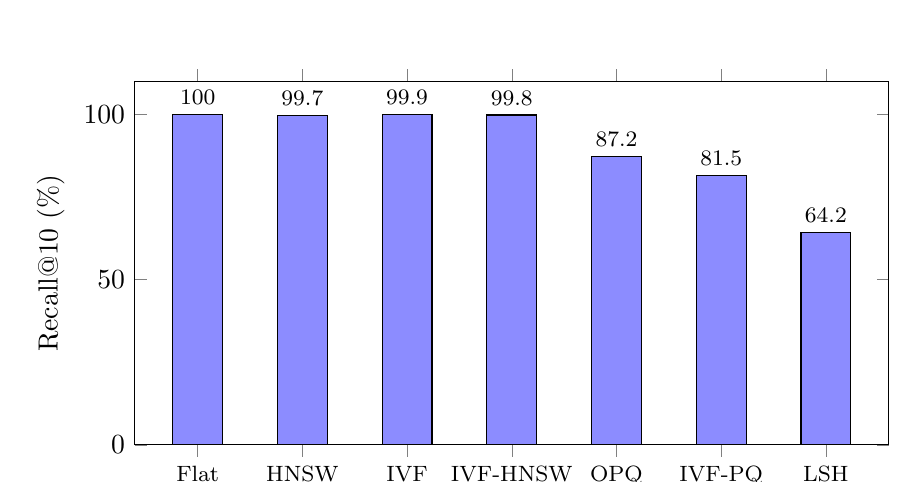
\begin{tikzpicture}
    \begin{axis}[
      width=0.92\textwidth,
      height=6.2cm,
      ybar,
      ymin=0,ymax=110,
      ylabel={Recall@10 (\%)},
      symbolic x coords={Flat,HNSW,IVF,IVF-HNSW,OPQ,IVF-PQ,LSH},
      xtick=data,
      nodes near coords,
      nodes near coords align={vertical},
      nodes near coords style={font=\footnotesize},
      bar width=18pt,
      enlarge x limits=0.10,
      x tick label style={font=\footnotesize}
    ]
      \addplot[fill=blue!45] coordinates {
        (Flat,100.0) (HNSW,99.7) (IVF,99.9) (IVF-HNSW,99.8)
        (OPQ,87.2) (IVF-PQ,81.5) (LSH,64.2)
      };
    \end{axis}
  \end{tikzpicture}
  \caption{各算法 Recall@10 对比}
\end{figure}

\begin{figure}[H]
  \centering
  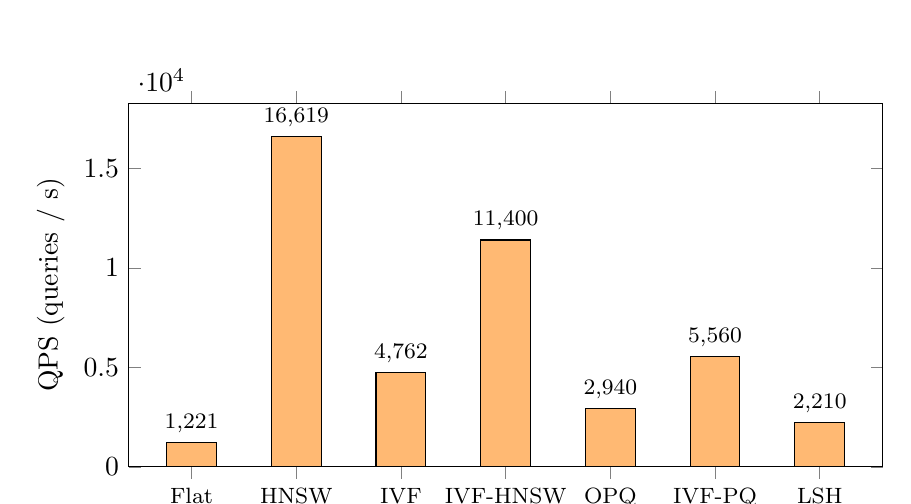
\begin{tikzpicture}
    \begin{axis}[
      width=0.92\textwidth,
      height=6.2cm,
      ybar,
      ymin=0,
      ylabel={QPS (queries / s)},
      symbolic x coords={Flat,HNSW,IVF,IVF-HNSW,OPQ,IVF-PQ,LSH},
      xtick=data,
      nodes near coords,
      nodes near coords align={vertical},
      nodes near coords style={font=\footnotesize},
      bar width=18pt,
      enlarge x limits=0.10,
      x tick label style={font=\footnotesize}
    ]
      \addplot[fill=orange!55] coordinates {
        (Flat,1221) (HNSW,16619) (IVF,4762) (IVF-HNSW,11400)
        (OPQ,2940) (IVF-PQ,5560) (LSH,2210)
      };
    \end{axis}
  \end{tikzpicture}
  \caption{各算法 QPS 吞吐对比}
\end{figure}

从结果看，可以得到以下几点结论：

\begin{itemize}
  \item \textbf{HNSW 适合默认交互检索。} 召回率（99.7\%）几乎逼近精确检索，但单条查询中位延迟约 0.06 ms，相对 Flat 提速约 13.6 倍，最适合 Web 工作台中即点即查的交互检索。
  \item \textbf{IVF 在召回与体积上表现均衡。} 召回率最高（99.9\%），索引体积也只有 9.4 MB，适合需要兼顾召回质量与存储成本的批量评测场景。
  \item \textbf{IVF-HNSW 折中召回与吞吐。} 在 IVF 的粗聚类基础上引入 HNSW，召回保持在 99.8\%，同时延迟和吞吐接近 HNSW，是 HNSW 与 IVF 之间一个有意义的折中选项。
  \item \textbf{量化与哈希族适合压缩场景。} IVF-PQ、OPQ 与 LSH 把索引压缩到 1$\sim$2 MB 级别，构建耗时增加，召回率下降到 60\%$\sim$90\%，适合内存受限或对存储压力敏感的部署环境。
  \item \textbf{Flat 仅作基线。} 在 69k 规模下还能维持毫秒级延迟，但 QPS 仅 1,221，规模继续放大时延迟线性上升，不适合作为生产环境的默认查询算法。
\end{itemize}

系统把上述指标结构化入库后，研究者可以根据数据规模、维度和业务目标自由选择算法，而不需要重新跑评测脚本。这也是本项目相对``只调用一个 ANN 库''的关键差异：评测结果可被沉淀、对比和复现。

为提供更丰富的视觉证据，建议补充以下两类对比图：

\begin{figure}[H]
  \centering
  \figplaceholder[5.5cm]{各算法延迟分位数对比图（p50 / p95 / p99）：横轴为算法名，纵轴为延迟（ms），可使用堆叠柱状图或多线图展示尾部延迟差异。}
  \caption{延迟分位数对比图（待补充）}
\end{figure}

\begin{figure}[H]
  \centering
  \figplaceholder[5.5cm]{各算法索引大小与构建耗时对比图：双坐标轴或并列柱状图，体现压缩算法（PQ/OPQ/LSH）的存储优势与构建成本。}
  \caption{索引大小与构建耗时对比图（待补充）}
\end{figure}

\begin{figure}[H]
  \centering
  \figplaceholder[6cm]{Recall--Latency 散点图：横轴为中位查询延迟（log 刻度），纵轴为 Recall@10，标注每个算法位置，可帮助研究者快速选择适合自己场景的算法。}
  \caption{Recall--Latency 折中图（待补充）}
\end{figure}

\section{验收测试清单}

\begin{longtable}{L{0.10\textwidth}L{0.38\textwidth}L{0.38\textwidth}}
  \caption{结项验收清单} \\
  \toprule
  编号 & 检查项 & 通过标准 \\
  \midrule
  \endfirsthead
  \toprule
  编号 & 检查项 & 通过标准 \\
  \midrule
  \endhead
  AC-01 & 项目可启动 & 后端 \texttt{/api/health} 返回 ok，前端可进入登录页。 \\
  AC-02 & 默认数据可用 & \texttt{liver} 数据集状态为 ready，细胞数、基因数和维度显示正确。 \\
  AC-03 & 索引可用 & HNSW 索引状态为 ready，可展示构建耗时和索引大小。 \\
  AC-04 & 基础检索通过 & 输入存在的 cell ID 后返回 Top-K，结果包含 cell ID、distance 和 obs。 \\
  AC-05 & 条件检索通过 & 增加 obs 条件后，返回 hit 的 obs 均满足条件。 \\
  AC-06 & 可视化通过 & 可加载 embedding 散点图，点击点位后右侧显示相似细胞。 \\
  AC-07 & Benchmark 通过 & 能创建评测批次并返回 recall、latency、QPS 等指标。 \\
  AC-08 & 导出通过 & CSV 可下载且包含表头和结果行。 \\
  AC-09 & 权限通过 & 未登录不能访问受保护页面，非管理员不能进入用户管理页。 \\
  AC-10 & 文档通过 & README、快速启动、报告和 slide 能说明安装、使用和设计。 \\
  \bottomrule
\end{longtable}

\section{质量控制}

项目的工程质量控制主要体现在以下方面：

\begin{itemize}
  \item \textbf{稳定 API 契约：} 前端只依赖明确的请求/响应字段，后端算法变化不影响页面。
  \item \textbf{服务层收敛复杂逻辑：} 路由层保持薄层，数据加载、索引构建、过滤和评测进入 service。
  \item \textbf{文件工件隔离：} 大型向量和索引文件不进入数据库，数据库只保存路径和状态。
  \item \textbf{显式状态机：} Dataset 和 Index 都有 ready、error、deleted 等状态，失败时保留 error message。
  \item \textbf{测试覆盖：} 合成数据测试避免依赖 1.4 GB 真实数据，提升 CI 和本地测试效率。
  \item \textbf{可观测结果：} 构建耗时、查询延迟、索引大小和 benchmark 结果均能在系统内查看或导出。
\end{itemize}

\chapter{项目管理}

本章从软件工程的角度，回顾项目在生命周期、工作分解、变更控制、配置管理、编码规范、集成发布、人员分工、进展记录、协作工具和风险管理等方面的具体做法。项目管理的目标，是在课程周期内既保证可运行系统按时交付，又留下可被复用和审查的过程资产。

\section{软件生命周期与过程模型}

本项目采用\textbf{迭代增量式}的软件开发过程。课程项目既需要在较短周期内形成可演示系统，又需要随着数据规模、算法支持、前后端联调和展示要求的变化不断补充功能。若采用一次性瀑布模型，早期很难完整确定 ANN 算法范围、过滤策略和前端交互细节；若完全不设阶段，则容易导致接口漂移和测试缺失。因此团队按``需求基线 $\to$ 架构基线 $\to$ 核心闭环 $\to$ 功能扩展 $\to$ 测试交付''的方式组织开发，每一轮迭代都形成可运行的功能增量。

\begin{longtable}{@{}L{0.13\textwidth}L{0.27\textwidth}L{0.28\textwidth}L{0.22\textwidth}@{}}
  \caption{软件生命周期阶段与主要产物} \\
  \toprule
  阶段 & 主要活动 & 阶段产物 & 质量门禁 \\
  \midrule
  \endfirsthead
  \toprule
  阶段 & 主要活动 & 阶段产物 & 质量门禁 \\
  \midrule
  \endhead
  需求分析 & 分析课程要求、单细胞检索场景、用户角色、核心功能和非功能指标。 & 功能需求表、需求追踪矩阵、典型用例、验收清单。 & 每个核心需求均能映射到接口、页面或测试项。 \\
  概要设计 & 确定前后端分离架构、数据工件方案、数据库表、API 契约和页面路由。 & 总体架构图、数据库表设计、接口表、UI 路由设计。 & 数据流从 \texttt{.h5ad} 到检索结果闭环清晰，模块职责不交叉。 \\
  详细设计 & 细化 Dataset Artifact、ANN Adapter、索引缓存、过滤策略、benchmark 和 RAG 模块。 & 模块职责表、算法参数表、请求响应示例、状态流转图。 & 关键模块有明确输入、输出、异常和状态变化。 \\
  编码实现 & 按模块实现后端 service/router/schema/model，前端实现 views、api、stores 和组件。 & 可运行前后端代码、默认数据引导、索引构建和检索页面。 & 本地启动通过，基础 API 可调用，前端主要页面可进入。 \\
  集成测试 & 联调登录、数据集、索引、检索、可视化、benchmark、导出和 RAG。 & Pytest/Vitest 测试、手工验收记录、benchmark 指标。 & 核心工作流不阻塞，错误路径可解释。 \\
  交付维护 & 整理 README、slide、报告、启动说明和后续改进方向。 & 结项报告、PDF、用户手册、风险清单、维护计划。 & 文档能支持第三方复现安装、运行和验收。 \\
  \bottomrule
\end{longtable}

\section{工作分解结构}

为了让开发任务可分配、可跟踪、可验收，项目按工作分解结构（Work Breakdown Structure, WBS）拆分为数据、算法、后端业务、前端界面、测试评估和文档交付六类工作包。每个工作包都尽量对应明确的代码目录或交付材料，避免只描述抽象职责。

\begin{longtable}{@{}L{0.12\textwidth}L{0.18\textwidth}L{0.42\textwidth}L{0.18\textwidth}@{}}
  \caption{项目工作分解结构} \\
  \toprule
  编号 & 工作包 & 工作内容 & 验收物 \\
  \midrule
  \endfirsthead
  \toprule
  编号 & 工作包 & 工作内容 & 验收物 \\
  \midrule
  \endhead
  WBS-01 & 数据接入 & 读取 \texttt{.h5ad}，抽取 embedding、cell ID 和 obs，生成可复用 Artifact。 & 数据集页面、预处理代码、样例 liver 数据记录。 \\
  WBS-02 & 索引算法 & 封装 Flat、HNSW、IVF、PQ、OPQ、LSH 等 ANN 算法，支持构建、加载和查询。 & ANN Adapter、factory、索引管理接口。 \\
  WBS-03 & 检索服务 & 实现按 cell ID、向量、批量、多数据集和组合索引检索，支持 Top-K 与过滤。 & \texttt{search} 模块、请求响应样例、检索页面。 \\
  WBS-04 & 评测分析 & 用 Flat 生成 ground truth，对算法的 recall、latency、QPS 和索引体积进行评估。 & benchmark 模块、评测页面、实验图表。 \\
  WBS-05 & 用户与权限 & 实现注册、登录、JWT 鉴权、角色权限、管理员审核和用户管理。 & auth/users 模块、登录页、用户管理页。 \\
  WBS-06 & 前端工作台 & 实现数据集、索引、检索、可视化、benchmark、导出、RAG 等页面。 & Vue views、API 封装、路由守卫。 \\
  WBS-07 & 可视化导出 & 展示二维/三维 embedding，支持点击联动检索和 CSV 导出。 & 可视化与导出模块、Plotly 组件。 \\
  WBS-08 & 文档交付 & 整理 README、快速启动、slide、结项报告和用户手册。 & 文档目录、PPT、LaTeX PDF 报告。 \\
  \bottomrule
\end{longtable}

\section{需求变更与评审机制}

课程项目在开发过程中不可避免会出现需求调整，例如从最初的单一 HNSW 检索扩展到多算法 benchmark、从单数据集检索扩展到多数据集检索、从普通搜索页面扩展到 RAG 辅助查询。项目采用轻量化变更控制机制：先判断变更是否影响既有 API 契约和数据库结构，再决定是否进入当前迭代。

\begin{itemize}
  \item \textbf{变更来源：} 课程要求、课堂汇报反馈、前后端联调问题、测试暴露的边界问题和展示体验优化。
  \item \textbf{影响分析：} 每项变更需判断是否影响数据库表、接口响应结构、前端页面状态、测试数据和文档说明。
  \item \textbf{优先级判断：} 影响主流程可用性的变更优先处理；加分扩展和体验优化在核心闭环稳定后处理。
  \item \textbf{回归检查：} 修改检索、索引或过滤逻辑后，需要重新检查基础检索、条件检索、benchmark 和导出路径。
  \item \textbf{文档同步：} 如果变更改变了启动方式、接口字段、页面入口或验收标准，README、报告和 slide 需要同步更新。
\end{itemize}

\section{配置管理与版本控制}

项目把源码、配置模板、文档和可复现脚本作为配置项管理，把大体积数据文件、数据库运行产物、索引文件和临时编译产物排除在版本控制之外。这样既能保证仓库可追踪，又避免 Git 历史被二进制大文件污染。

\begin{longtable}{@{}L{0.18\textwidth}L{0.36\textwidth}L{0.36\textwidth}@{}}
  \caption{配置项管理策略} \\
  \toprule
  配置项类别 & 管理对象 & 控制策略 \\
  \midrule
  \endfirsthead
  \toprule
  配置项类别 & 管理对象 & 控制策略 \\
  \midrule
  \endhead
  源代码 & \texttt{backend/app}、\texttt{frontend/src}、测试代码。 & 使用 Git 记录变更，功能按模块提交，避免无关格式化混入业务修改。 \\
  依赖配置 & \texttt{environment.yml}、\texttt{package.json}、\texttt{requirements.txt}。 & 依赖变更需能解释用途，避免引入未使用库。 \\
  运行配置 & \texttt{.env.example}、后端和前端环境变量说明。 & 提供模板和文档，不提交真实密钥、token 或个人路径。 \\
  数据工件 & \texttt{vectors.npy}、\texttt{cell\_ids.npy}、\texttt{obs.parquet}、ANN index 文件。 & 由系统运行生成，数据库只记录路径和状态，交付时不强制纳入 Git。 \\
  文档材料 & README、快速启动、设计文档、slide、report。 & 与功能变更同步更新，报告保留 \texttt{tex} 源码和最终 PDF。 \\
  临时产物 & \texttt{aux}、\texttt{log}、\texttt{toc}、页面检查图片、构建缓存。 & 编译和检查后清理，不作为最终交付文件。 \\
  \bottomrule
\end{longtable}

\section{编码规范与设计原则}

项目代码遵循分层、清晰、可测试的原则。后端把模型、schema、router、service 和算法 adapter 分开，前端把页面、API 封装、状态管理和复用组件分开，避免把数据访问、业务逻辑和展示逻辑混在同一文件中。

\begin{itemize}
  \item \textbf{接口优先：} 前后端以稳定 JSON 契约为边界，响应字段命名保持一致，错误信息可直接展示。
  \item \textbf{薄路由厚服务：} FastAPI router 负责参数接收和权限依赖，数据处理、索引生命周期和检索策略放入 service。
  \item \textbf{算法可替换：} 所有 ANN 算法通过统一 Adapter 暴露 \texttt{build}、\texttt{search}、\texttt{save}、\texttt{load} 等能力。
  \item \textbf{状态显式：} Dataset、Index、CombinedIndex 和 BenchmarkBatch 均保存状态字段，前端不依赖隐式文件存在性判断。
  \item \textbf{异常可恢复：} 构建失败、维度不匹配、cell ID 不存在、外部模型不可用等情况均返回明确错误。
  \item \textbf{组件复用：} 前端通用表格、表单、状态标签、API 请求和路由守卫集中封装，减少重复逻辑。
  \item \textbf{测试友好：} 后端测试使用合成小型 AnnData 和临时 SQLite，避免依赖真实大文件，降低本地和 CI 成本。
\end{itemize}

\section{集成、发布与维护计划}

项目交付不只关注代码能否运行，还需要定义从开发到验收的集成路径。课程阶段采用本地部署和手工验收为主；后续若进入长期维护，可引入 CI、后台任务队列、生产数据库和统一日志监控。

\begin{longtable}{@{}L{0.18\textwidth}L{0.40\textwidth}L{0.32\textwidth}@{}}
  \caption{集成发布与维护计划} \\
  \toprule
  环节 & 执行内容 & 检查点 \\
  \midrule
  \endfirsthead
  \toprule
  环节 & 执行内容 & 检查点 \\
  \midrule
  \endhead
  本地集成 & 后端启动 FastAPI，前端通过 \texttt{VITE\_API\_BASE} 连接真实接口。 & 登录、数据集、索引和检索主流程可操作。 \\
  自动化验证 & 运行 Pytest、Vitest 和前端生产构建。 & 测试通过，TypeScript 构建无阻塞错误。 \\
  数据初始化 & 通过 bootstrap 注册 liver 数据集并构建默认 HNSW 索引。 & 数据集和索引状态均为 ready，维度一致。 \\
  演示验收 & 按验收清单执行登录、检索、过滤、可视化、benchmark、导出。 & 每个 AC 条目有对应页面或接口证据。 \\
  文档发布 & 更新 README、报告、用户手册和 PPT。 & 安装步骤、默认账号、配置项和注意事项一致。 \\
  运行维护 & 定期清理失败索引、临时 benchmark 结果和过期导出文件。 & 磁盘空间可控，数据库状态与文件系统一致。 \\
  后续演进 & 引入 Celery/RQ、PostgreSQL、Alembic、对象存储和服务监控。 & 长任务可追踪，部署环境可迁移，数据资产可备份。 \\
  \bottomrule
\end{longtable}

\section{参与人员及分工}

下表根据 Git 提交作者记录与项目模块整理，正式提交前可替换为课程要求的真实姓名、学号和贡献度。

\begin{table}[H]
  \centering
  \caption{参与人员记录与模块分工}
  \begin{tabularx}{0.95\textwidth}{lY}
    \toprule
    Git 作者 & 主要参与方向 \\
    \midrule
    \texttt{sjq0098} & 后端环境、数据集、索引、ANN、检索和项目进度记录等模块。 \\
    \texttt{Wei Lai} & 前后端集成、后端功能扩展、RAG、benchmark、组合索引和联调修复。 \\
    \texttt{hqz} & 前端页面、工作台布局、交互组件和界面修复。 \\
    \texttt{Sasuke-CS} & 前端功能页、视觉统一、数据集/检索/可视化页面与演示体验。 \\
    \texttt{2311671-Hou Jiadong} & 前端功能补充、接口联调、文档和演示材料。 \\
    \bottomrule
  \end{tabularx}
\end{table}

\section{项目进展记录}

项目使用 Git 管理开发过程，远程仓库为 \href{https://github.com/wl-8/scann-search}{scann-search GitHub 仓库}。提交记录显示项目经历了后端 ANN 算法实现、前端工作台重构、联调修复、benchmark/RAG/组合索引扩展和最终界面统一等阶段。典型提交包括：

\begin{itemize}
  \item \texttt{feat: add ann benchmark, combined index, and rag}
  \item \texttt{feat(frontend): align new features with polish workbench}
  \item \texttt{feat: overhaul frontend UI consistency and polish across all pages}
  \item \texttt{feat: connect dashboard to liver dataset}
  \item \texttt{debug for cosine metrics and update cache}
\end{itemize}

\begin{figure}[H]
  \centering
  \figplaceholder[5cm]{GitHub 提交历史截图：建议截取仓库 \texttt{commits} 页面或 \texttt{git log --graph --oneline} 输出，体现项目演进脉络与多位作者的协作记录。}
  \caption{Git 提交历史（待补充）}
\end{figure}

\begin{figure}[H]
  \centering
  \figplaceholder[4.5cm]{GitHub 贡献者图：建议截取仓库 Contributors 页面或 \texttt{git shortlog -s -n} 结果，量化呈现各成员的提交次数和代码贡献。}
  \caption{贡献者统计（待补充）}
\end{figure}

\section{项目管理工具}

\begin{itemize}
  \item \textbf{Git/GitHub：} 用于版本控制、远程同步和提交记录追踪。
  \item \textbf{Markdown 文档：} \texttt{README.md}、\texttt{快速启动.md}、前后端设计文档和对接清单用于同步开发约定。
  \item \textbf{进度日志：} \texttt{progress.md} 记录后端 ANN 开发目标、改前状态、改后状态和涉及文件。
  \item \textbf{PPT：} \texttt{slide/团队作业.pptx} 和 \texttt{slide/软件工程\_scann-search\_PPT(1).pptx} 用于课程展示和结项汇报。
  \item \textbf{自动化测试：} Pytest 和 Vitest 用于验证核心模块行为，降低联调风险。
\end{itemize}

\section{风险管理}

\begin{longtable}{L{0.20\textwidth}L{0.34\textwidth}L{0.34\textwidth}}
  \caption{项目风险与应对措施} \\
  \toprule
  风险 & 表现 & 应对措施 \\
  \midrule
  \endfirsthead
  \toprule
  风险 & 表现 & 应对措施 \\
  \midrule
  \endhead
  二进制依赖安装失败 & FAISS、hnswlib、Scanpy 在 Windows pip 环境下编译失败。 & 提供 \texttt{environment.yml}，优先使用 conda-forge 预编译包。 \\
  大数据文件过大 & \texttt{.h5ad} 体积可达 GB 级，直接入库或提交 Git 不现实。 & Git 忽略大文件，系统只保存路径和轻量 Artifact。 \\
  索引与向量不一致 & 切换 embedding 后旧索引维度与新向量不匹配。 & embedding 切换时级联删除旧索引，检索前校验维度。 \\
  条件过滤召回不足 & 稀有细胞类型过滤时 post-filter 返回不足 Top-K。 & 提供 oversample、pre-filter、hybrid 策略对比。 \\
  前后端字段漂移 & 页面字段名与后端 schema 不一致导致联调失败。 & 维护前后端对接清单，接口封装集中在 \texttt{src/api}。 \\
  长任务阻塞 & 大数据集构建索引或 benchmark 请求耗时较长。 & 课程阶段同步实现，后续规划后台任务队列。 \\
  RAG 外部依赖不可用 & API key 未配置或外部模型服务失败。 & 提供 local provider，至少返回本地证据摘要。 \\
  \bottomrule
\end{longtable}

\chapter{用户手册}

本章面向首次部署或使用 \project 的用户，按照``安装启动 $\to$ 主要操作流程 $\to$ 注意事项 $\to$ 常见问题''的顺序给出步骤化说明。其中安装启动部分针对课程演示环境进行了简化，更复杂的生产部署请参考第 5 章的集成发布与维护计划。

\section{安装与启动}

后端推荐使用 conda 环境，以避免 Windows 或 WSL 下 FAISS、Scanpy、hnswlib 等二进制依赖编译失败。

\subsection{环境变量配置}

后端启动前需要在 \texttt{backend/.env} 中配置必要变量。最小配置如下：

\begin{lstlisting}[caption={后端 .env 最小配置}]
SECRET_KEY=change-me
ADMIN_PASSWORD=Admin@123456
DATABASE_URL=sqlite:///./app.db
UPLOAD_DIR=data/uploads
INDEX_DIR=data/indexes
AUTO_BOOTSTRAP_DATA=true
BOOTSTRAP_DATASET_NAME=liver
BOOTSTRAP_DATASET_PATH=data/liver.h5ad
BOOTSTRAP_EMBEDDING_KEY=X_pca
BOOTSTRAP_INDEX_ALGORITHM=hnsw
\end{lstlisting}

上述前几项分别控制 JWT 签名密钥、默认管理员密码、上传工件目录和索引目录。若启用外部大模型，可额外配置 OpenAI、DeepSeek 等 provider 对应的 API key。

\Needspace{13\baselineskip}
\subsection{后端启动}

\begin{lstlisting}[language=bash,caption={后端启动}]
conda env create -f environment.yml
conda activate scann-search
cd backend
uvicorn app.main:app --reload --host 127.0.0.1 --port 8000
\end{lstlisting}

如果已经具备 Python 环境，也可以使用 pip 安装纯 Python 依赖：

\begin{lstlisting}[language=bash,caption={后端 pip 安装}]
cd backend
pip install -r requirements.txt
uvicorn app.main:app --reload
\end{lstlisting}

\subsection{前端启动}

前端启动方式如下：

\begin{lstlisting}[language=bash,caption={前端启动}]
cd frontend
npm install
npm run dev
\end{lstlisting}

如果需要连接真实后端，在 \texttt{frontend/.env} 中配置：

\begin{lstlisting}[caption={前端环境变量}]
VITE_API_BASE=http://localhost:8000/api
\end{lstlisting}

启动后访问 Vite 输出的地址，例如 \url{http://localhost:5173/}。默认管理员账号可参考项目快速启动文档：用户名 \texttt{admin}，密码 \texttt{Admin@123456}。

\subsection{启动后检查}

建议按以下顺序检查系统是否正确运行：

\begin{enumerate}
  \item 访问 \texttt{http://localhost:8000/api/health}，确认返回 \texttt{\{"status":"ok"\}}。
  \item 打开前端登录页，使用管理员账号登录。
  \item 进入数据集页面，确认默认 \texttt{liver} 数据集状态为 ready。
  \item 进入索引页面，确认至少存在一个 ready 索引；若不存在，选择数据集和 HNSW 算法构建。
  \item 进入检索页，选择 ready 索引，输入存在的 cell ID 或向量，确认可返回 Top-K。
  \item 进入可视化页，加载散点图并点击点位，确认检索结果联动展示。
\end{enumerate}

\section{主要操作流程}

本节按``登录 $\to$ 数据集 $\to$ 索引 $\to$ 检索 $\to$ 可视化 $\to$ 评测 $\to$ RAG $\to$ 导出''的顺序，给出每个核心操作的步骤说明。每一节均预留了对应页面截图位置，建议在最终交付版本中替换为真实运行截图。

\subsection{登录系统}

打开 \texttt{/login}，输入账号密码后登录。登录成功后前端保存 token，并请求 \texttt{/auth/me} 获取用户信息。如果账号未审核、被禁用或密码错误，系统会显示错误提示。

\begin{figure}[H]
  \centering
  \figplaceholder[4cm]{登录页操作截图：用户名 / 密码填写、登录按钮点击和登录成功后跳转仪表盘的画面。}
  \caption{登录系统操作截图（待补充）}
\end{figure}

\subsection{注册数据集}

进入数据集管理页，选择上传文件或填写服务器上的 \texttt{.h5ad} 路径，输入数据集名称和 embedding key，例如 \texttt{X\_pca}。提交后后端读取 AnnData，抽取 vectors、cell IDs 和 obs，并将数据集状态置为 ready。若 embedding key 不存在或文件无法读取，状态会变为 error 并返回错误信息。

\begin{figure}[H]
  \centering
  \figplaceholder[5cm]{注册数据集操作截图：上传 / 路径填写表单，提交后状态从 processing 切换到 ready 的画面。}
  \caption{注册数据集操作截图（待补充）}
\end{figure}

\subsection{构建索引}

进入索引管理页，选择 ready 数据集和算法。HNSW 可使用默认参数，也可以自定义：

\begin{lstlisting}[caption={HNSW 参数示例}]
{
  "M": 16,
  "ef_construction": 200,
  "ef_search": 50
}
\end{lstlisting}

构建成功后，页面会显示算法、状态、向量数量、维度、构建耗时和索引大小。

\begin{figure}[H]
  \centering
  \figplaceholder[5cm]{构建索引操作截图：算法选择、参数表单、构建中状态以及构建完成后展示 build\_time\_ms 与 index\_size 的画面。}
  \caption{构建索引操作截图（待补充）}
\end{figure}

\subsection{相似细胞检索}

进入检索页，选择数据集和索引，输入查询 cell ID 或向量，设置 Top-K 和过滤条件。系统返回相似细胞列表，包含 rank、cell ID、row index、distance 和 obs 元数据。若启用条件过滤，返回结果只保留满足条件的细胞。

\begin{figure}[H]
  \centering
  \figplaceholder[5.5cm]{相似细胞检索操作截图：输入示例 cell ID（如 \texttt{AAACCTGAG...}），返回 Top-10 结果表格、延迟、过滤条件等信息。}
  \caption{相似细胞检索操作截图（待补充）}
\end{figure}

\subsection{可视化联动检索}

进入可视化页，选择数据集、展示模式和着色字段，加载 embedding 散点图。点击任意细胞点后，页面会显示该细胞的元数据，并自动以该细胞作为查询发起相似检索。

\begin{figure}[H]
  \centering
  \figplaceholder[6cm]{可视化联动检索操作截图：左侧 Plotly 散点图（按 cell\_type 着色），点击某细胞后右侧弹出 metadata 与相似细胞列表的联动效果。}
  \caption{可视化联动检索操作截图（待补充）}
\end{figure}

\subsection{运行性能评测}

进入性能评测页，选择数据集、Top-K、查询数量、随机种子和多个算法配置。系统使用 Flat 生成 ground truth，并对每个算法计算 recall、latency、QPS、构建耗时和索引大小。评测结果可以在页面查看，也可以导出 CSV。

\begin{figure}[H]
  \centering
  \figplaceholder[5.5cm]{运行性能评测操作截图：算法多选 + Top-K / queries / seed 表单 + 评测结果图表（Recall / Latency / QPS）。}
  \caption{运行性能评测操作截图（待补充）}
\end{figure}

\subsection{RAG 自然语言查询}

进入 RAG 页面，输入问题，例如``查询健康肝脏样本中与某类细胞相似的细胞''。系统会结合过滤条件和数据集证据生成回答。若未配置外部模型 API key，系统仍可以返回本地证据摘要。

\begin{figure}[H]
  \centering
  \figplaceholder[5.5cm]{RAG 自然语言查询操作截图：自然语言提问、解析得到的过滤条件、数据证据摘要、模型最终回答以及 provider 信息。}
  \caption{RAG 自然语言查询操作截图（待补充）}
\end{figure}

\subsection{导出结果}

进入导出页面后，可以选择导出检索结果、过滤结果或 benchmark 结果。导出的 CSV 可用于 Excel、Python、R 或论文图表制作。建议在导出后检查表头是否包含 cell ID、distance、obs 字段或 benchmark 指标字段。

\begin{figure}[H]
  \centering
  \figplaceholder[4cm]{导出结果操作截图：导出类型选择、下载按钮、以及在 Excel / 文本编辑器中打开 CSV 的对比效果。}
  \caption{导出结果操作截图（待补充）}
\end{figure}

\section{操作注意事项}

\begin{itemize}
  \item 注册数据集时，embedding key 必须存在于 AnnData 的 \texttt{obsm} 中；若使用 \texttt{X\_umap} 等低维 embedding，后续跨数据集检索必须保证维度一致。
  \item 构建 HNSW 时，如果更重视召回率，可以增大 \texttt{ef\_search}；如果更重视响应速度，可以适当降低该参数。
  \item 条件过滤选择率很低时，post-filter 可能返回不足 Top-K；可以增大 oversample 或使用策略对比页面观察 pre/hybrid 效果。
  \item Benchmark 会临时构建索引并执行多次查询，查询数量越大结果越稳定，但耗时也越长。
  \item RAG 外部模型需要 API key；未配置时可使用 local 模式生成本地证据摘要。
\end{itemize}

\section{常见问题}

\begin{table}[H]
  \centering
  \caption{常见问题与处理方式}
  \begin{tabularx}{0.95\textwidth}{lY}
    \toprule
    问题 & 处理方式 \\
    \midrule
    前端页面空白 & 确认在 \texttt{frontend} 目录执行 \texttt{npm run dev}，并查看浏览器控制台错误。 \\
    前端提示后端资源加载失败 & 检查 FastAPI 是否运行在 \texttt{8000} 端口，以及 \texttt{VITE\_API\_BASE} 是否正确。 \\
    后端启动时报缺少 \texttt{SECRET\_KEY} 或 \texttt{ADMIN\_PASSWORD} & 在 \texttt{backend/.env} 中按 \texttt{.env.example} 配置必需变量。 \\
    FAISS 或 hnswlib 安装失败 & 优先使用 \texttt{environment.yml} 通过 conda-forge 安装预编译包。 \\
    搜索返回维度不匹配 & 确认查询向量维度与索引的 \texttt{vector\_dim} 一致，跨数据集检索需统一 embedding 维度。 \\
    条件过滤返回结果不足 Top-K & 过滤选择率较低时可增大 oversample，或使用 pre/hybrid 过滤策略。 \\
    Benchmark 时间较长 & 减少 \texttt{n\_queries} 或算法数量；大规模评测建议后续迁移到后台任务队列。 \\
    \bottomrule
  \end{tabularx}
\end{table}

\chapter{总结与展望}

\section{项目总结}

\project 已完成一个可运行的单细胞 ANN 检索 Web 系统。系统从 \texttt{.h5ad} 数据注册开始，经过 Dataset Artifact 落盘、ANN 索引构建、Top-K 检索、条件过滤、可视化联动、性能评测和结果导出，形成了一条较完整的单细胞向量检索研究工作流。在课程层面，项目不仅实现了中期要求的单细胞数据读取、向量化表示、ANN 索引构建和相似细胞检索，也覆盖了结项要求中的条件检索、性能评估、可视化展示、数据集管理与动态索引管理，并进一步尝试了多数据集联合检索、组合索引、ANN 算法对比和 RAG 自然语言辅助分析等加分方向。

项目的主要亮点可以归纳为以下六点：

\begin{itemize}
  \item \textbf{面向单细胞场景的数据流。} 围绕 cell ID、embedding 和 obs 元数据组织检索流程，结果直接可被生物学解释。
  \item \textbf{Dataset Artifact 抽象。} 将大文件解析与在线检索解耦，向量、cell ID 和 obs 行号严格对齐，提升复用性和响应速度。
  \item \textbf{ANN Adapter 抽象。} 屏蔽 Flat、HNSW、IVF、PQ、OPQ、LSH、IVF-PQ、IVF-HNSW 等 8 种算法的实现差异，新增算法不需要修改 API 契约。
  \item \textbf{统一条件过滤语义。} 数据浏览、检索、策略对比、benchmark、导出和 RAG 证据收集共享同一过滤模型。
  \item \textbf{Benchmark 评测闭环。} 以 Flat 精确检索为 ground truth，结构化记录 Recall、Latency、QPS、Build Time 和 Index Size，支持可复现实验。
  \item \textbf{完整 Web 工作台。} 前端提供从登录、数据集、索引、检索到可视化、评测、导出和 RAG 的完整后台，便于课程展示与非工程背景研究者使用。
\end{itemize}

从《软件工程》课程视角看，项目较为完整地呈现了``需求分析$\to$系统设计$\to$编码实现$\to$测试评估$\to$项目管理$\to$文档交付''全过程，并通过 Git 提交历史、PPT 汇报和本报告对开发过程进行了沉淀。

\section{不足与改进方向}

囿于课程周期与团队规模，项目仍有以下值得继续推进的方向：

\begin{itemize}
  \item \textbf{异步任务化。} 数据集预处理、索引构建和 benchmark 目前以同步请求为主，大规模数据场景下应迁移到 Celery/RQ 等任务队列，并补充进度查询、失败重试和取消能力。
  \item \textbf{生产数据库支持。} 当前开发阶段使用 SQLite，后续可迁移到 PostgreSQL，并通过 Alembic 管理 schema 演进，配合连接池和读写分离。
  \item \textbf{参数自动推荐。} 可根据数据规模、维度、过滤选择率和目标召回，自动推荐 HNSW/IVF 等算法的关键参数，降低研究者上手成本。
  \item \textbf{过滤索引优化。} 对高频 obs 字段建立倒排或位图索引，使 pre-filter 与 hybrid filter 在低选择率条件下更稳定。
  \item \textbf{更广的真实评测。} 增加多数据集、多 embedding 维度和不同细胞类型过滤条件下的 benchmark 对比图表，并把结果直接绑定到前端图表组件中。
  \item \textbf{RAG 上下文深化。} 把检索命中细胞、元数据分布、可视化位置和 benchmark 结果组织成更结构化的解释上下文，使 RAG 回答更接近研究助手的角色。
  \item \textbf{可观测性。} 增加任务日志、耗时追踪、资源占用监控和导出历史管理，方便后续运维与问题排查。
\end{itemize}

\chapter*{参考文献}
\addcontentsline{toc}{chapter}{参考文献}

\begin{enumerate}
  \item Malkov, Y. A., and Yashunin, D. A. Efficient and robust approximate nearest neighbor search using Hierarchical Navigable Small World graphs. IEEE TPAMI, 2020.
  \item Johnson, J., Douze, M., and Jegou, H. Billion-scale similarity search with GPUs. IEEE Transactions on Big Data, 2019.
  \item Wolf, F. A., Angerer, P., and Theis, F. J. SCANPY: large-scale single-cell gene expression data analysis. Genome Biology, 2018.
  \item Virshup, I. et al. The scverse project provides a computational ecosystem for single-cell omics data analysis. Nature Biotechnology, 2023.
\end{enumerate}

\end{document}
